\chapter{Exploring topological sensitivity}\label{ch:exploring-topological-sensitivity}

In the previous chapter, I discussed data concerning quantification over parts in explicit entity and set partitives. Specifically, I presented  evidence suggesting that only integrated parts of integrated wholes can be subject to counting. As I have already indicated in the introduction, in English the difference can be captured by the contrast between bare \textit{part} and \textit{a part}. I argued that expressions corresponding to the former refer to arbitrary parts of a whole including discontinuous portions of a substance making up a whole, and thus are uncountable. On the other hand, expressions corresponding to the latter refer to continuous integrated parts of a whole and as such can pluralize and combine with cardinals. In this chapter, I explore to what extent natural language is sensitive to this distinction. To this end, I will provide novel evidence from different types of Polish partitive words that encode the contrast formally. It will turn out that this phenomenon is not something idiosyncratic, but rather cross-linguistic evidence suggests that it is relatively widespread with different languages using different means to express it. Moreover, based on the data concerning whole-adjectives I will demonstrate the linguistic relevance of two aspects of being whole, namely maximality and integrity.\footnote{The scope of this chapter would be much narrower if it were not for my informants with whom I tested the interpretation of expressions in languages other than Polish. In particular, I am very grateful to Jonathan Bobaljik, Jeffrey Parrott, and Guy Tabachnick for their judgments and discussion concerning English, to Berit Gehrke, Nina Haslinger, and Maximilian Prüller for German, Erlinde Meertens and Izabela Jordanoska for Dutch, Muriel Assmann for Brazilian Portuguese, and Chang Liu for Mandarin. I would also like to thank Adam Przepiórkowski for sharing his observations regarding Polish with me.}

\section{Continuous and discontinuous parts}\label{sec:continuous-discontinuous-parts}

Given the meaning of the plural in languages such as English, it follows that expressions such as \textit{a part} are incompatible with predicates denoting pluralities. Intuitively, the reason is that the extension of a phrase headed by \textit{a part} comprises integrated portions, i.e., parts that come in one piece, whereas plurals denote arbitrary sums, i.e., scattered entities consisting of discontinuous elements. However, if the plural were augmented with an additional semantic feature guaranteeing that a plurality of integrated objects is itself an integrated object, as is arguably the case in at least some Italian irregular plurals, then an expression corresponding to English \textit{a part} is able to combine with such a plural expression. In such a case, it would yield a part of a plurality whose constituents are in a particular topological relation, namely they are connected to each other.

But is there any additional reason to assume that natural language expressions are sensitive to topological relations operating alongside part-whole structures? And if so, to what extent do the discussed phenomena really tell us something important about countability? The claim advanced here is that what counts as one needs to be an integrated part (proper or improper) of an integrated whole. Though this might seem intuitively correct, a question arises where the property of `coming in one piece' comes from. After all, countability is the ability of an expression to appear in morpho-syntactic environments related to counting, but counting is a semantic operation of assigning numbers to units of a particular type. Hence, one could wonder whether there is evidence that there is something in an expression's meaning that corresponds to the notion of being an integrated entity, and thus being countable. One prominent view holds that countability is not a property of a particular class of nouns but rather of full DPs (e.g., \citealt{borer2005name}, see also \citealt{allan1980nouns} and \citealt{pelletier_schubert1989mass} and the following work by \citeauthor{pelletier2011descriptive}), and thus arises within a complex nominal syntactic structure. On the other hand, other approaches posit that it is lexical meaning that determines countability patterns  \citep[e.g.,][]{wierzbicka1988semantics,wisniewski_lamb_middleteon2003conceptual}. However, the evidence discussed in the literature is mainly restricted to cases of quantification over wholes and almost totally ignores constructions in which what is counted are bits of objects rather than whole individuals.

In this section, I will provide additional evidence for the significance of the role of spatial integrity, i.e., compactness, of parts in subatomic quantification. The core data come from the distribution and semantic properties of distinct classes of Polish half-words.

\subsection{Polish half-words}\label{sec:polish-half-words}

Polish distinguishes lexically between three distinct half-words, as presented in \ref{ex:polish-half-words-morphology}. They are morphologically derived from one another with \textit{pół} being morphologically the least marked form with no derivational affixes. As presented in \ref{ex:polish-half-pol-morphology}, \textit{pół} consists only of a root and null inflectional marker. On the other hand, \textit{połowa} and \textit{połówka} are derived forms involving in addition the morpheme \textit{-ow-/-ów-} as well as the diminutive suffix \textit{-k-} in the latter case, see \ref{ex:polish-half-polowa-morphology}--\ref{ex:polish-half-polowka-morphology}.

		\ex. Polish\label{ex:polish-half-words-morphology}
        \ag. pół-$\varnothing$\\
		root-inflectional.marker\\
		`half$_1$'\label{ex:polish-half-pol-morphology}
		\bg. poł-ow-a\\
		root-derivational.suffix-inflectional.marker\\
		`half$_2$'\label{ex:polish-half-polowa-morphology}
        \bg. poł-ów-k-a\\
		root-deriv.suffix$_1$-deriv.suffix$_2$-infl.marker\\
		`half$_3$'\label{ex:polish-half-polowka-morphology}

In terms of $\phi$-features, \textit{pół} shows neuter agreement whereas \textit{połowa} and \textit{połówka} are feminine, as demonstrated in \ref{ex:polish-half-words-agreement}. Furthermore, similarly to vague quantifiers such as \textit{dużo} `many/much', \textit{pół} is defective in that it has only the nominative/accusative form (though it can also appear in some genitive positions).\footnote{\label{fn:plural-pol}Based on examples from the National Corpus of Polish (NCP) like \ref{ex:inherent-plural}, \citet{przepiorkowski2006inherentnej} argues that \textit{pół} `half' is inherently plural because it can be modified by the plural demonstrative \textit{te} `these'. Notice, however, that though there are definitely varieties of Polish in which \ref{ex:inherent-plural} is well-formed, there are also many speakers (including myself) for whom it is ungrammatical. Furthermore, in modern Polish the neuter singular demonstrative \textit{to} `this' is being gradually replaced by the colloquial form \textit{te} `this' which is homophonous to the plural \textit{te} `these'. It is possible that the acceptability of \ref{ex:inherent-plural} is correlated with this process.

\ex. Polish (NCP)
\bg.[] \%Zaczną się niebawem prace polowe, więc te pół kilometra jest konieczne.\\
will.begin \textsc{refl} soon works field.\textsc{adj} so these half kilometer.\textsc{gen} is necessary\\
`Field work will start soon, so it is necessary (to finish) this half kilometer (road).'\label{ex:inherent-plural}

}\largerpage[2]

\ex. Polish\label{ex:polish-half-words-agreement}
\ag. To czerwone pół jabłka zgniło.\\
this\textsc{.nom.n} red\textsc{.nom.sg.n} half$_{1}$\textsc{.nom.n} apple\textsc{.gen.n} rotted\textsc{.sg.n}\\
`This red half of the apple got spoiled.'
\bg. Ta czerwona połowa jabłka zgniła.\\
this\textsc{.nom.f} red\textsc{.nom.sg.f} half$_{2}$\textsc{.nom.f} apple\textsc{.gen.n} rotted\textsc{.sg.f}\\
`This red half of the apple got spoiled.'
\bg. Ta czerwona połówka jabłka zgniła.\\
this\textsc{.nom.f} red\textsc{.nom.sg.f} half$_{3}$\textsc{.nom.f} apple\textsc{.gen.n} rotted\textsc{.sg.f}\\
`This red half of the apple got spoiled.'

At first blush, the Polish half-words in \ref{ex:polish-half-words-agreement} are mere synonyms making the same contribution to the interpretation of the discussed sentences. However, closer investigation reveals intriguing differences in their distribution and meaning. Let us first consider the most frequent and semantically least marked \textit{half} expression, i.e., \textit{połowa}. As witnessed in \ref{ex:distribution-polowa}, there are no constraints on its distribution and it can felicitously combine with all types of entity-denoting predicates including count singulars, collectives, plurals, and mass terms.\footnote{In this section, I provide the examples with collective nouns only for the sake of completeness, i.e., in order to show the distributional difference between \textit{pół} and \textit{połówka}. In the remaining part of this chapter (except of \sectref{sec:quarter-words}), I will not investigate the interaction between partitives and collectives.}
		
		\ex. Polish\label{ex:distribution-polowa}
        \ag. połowa jabłka\\
		half$_2$ apple\textsc{.gen}\\
		`half of the apple'\label{ex:distribution-polowa-sg}
		\bg. połowa  stosu (jabłek)\\
		half$_2$ pile\textsc{.gen} (apples\textsc{.gen})\\
		`half of the pile (of apples)'\label{ex:distribution-polowa-group}
		\bg. połowa jabłek\\
		half$_2$ apples\textsc{.gen}\\
		`half of the apples'\label{ex:distribution-polowa-pl}
		\bg. połowa soku\\
		half$_2$ juice\textsc{.gen}\\
		`half of the juice'\label{ex:distribution-polowa-mass}

On the other hand, \textit{pół} has a more restricted distribution since it is incompatible with cumulative predicates such as plurals and mass nouns, see \ref{ex:distribution-pol}. Thus, it can only combine with regular count singulars and collective nouns.\largerpage
		
		\ex. Polish\label{ex:distribution-pol}
        \ag. pół jabłka\\
		half$_1$ apple\textsc{.gen}\\
		`half of the apple'\label{ex:distribution-pol-sg}
		\bg. pół stosu \minsp{(} jabłek)\\
		half$_1$ pile\textsc{.gen} {} apples\textsc{.gen}\\
		`half of the pile (of apples)'\label{ex:distribution-pol-group}
		\bg. \# pół jabłek\\
		half$_1$ apples\textsc{.gen}\label{ex:distribution-pol-pl}\\
		Intended: `half of the apples'
		\bg. \# pół soku\\
		half$_1$ juice\textsc{.gen}\label{ex:distribution-pol-mass}\\
		Intended: `half of the juice'

Notice that the constraint on the distribution of \textit{pół} is not morpho-syntactic. The phrases in \ref{ex:pl.tantum-pol} show that it can felicitously combine with pluralia tantum. However, in such a case the whole partitive phrase gets a part-of-a-singularity interpretation. Specifically, \ref{ex:pl.tantum-pol-scissors} cannot refer to 50\% of the relevant utensils but only to a half of one pair of scissors. In a similar vein, \ref{ex:pl.tantum-pol-dried-fruit} involves the noun \textit{bakalie} `dried fruit' which is a plurale tantum expression in Polish and as such it can either denote one piece of dried fruit or a plurality thereof. The half-word \textit{pół} can combine with \textit{bakalie} as long as it quantifies over material parts of a single foodstuff. For instance, it would be true of a half of a raisin but not of, say, five out of ten raisins. 

	\ex. Polish\label{ex:pl.tantum-pol}
    \ag. pół nożyczek\\ 
	half$_1$ scissors\textsc{.gen}\\
	`half of the scissors'\label{ex:pl.tantum-pol-scissors}
	\bg. pół bakalii\\ 
	half$_1$ dried.fruit\textsc{.gen.pl}\\
	`half of the dried fruit'\label{ex:pl.tantum-pol-dried-fruit}

Furthermore, the claim that \textit{pół} is incompatible with mass nouns is somewhat imprecise and requires elaboration. In fact, when it can combine with mass terms, it enforces a mass-count shift via the Universal Packager \citep[see, e.g.,][]{bach1986algebra,jackendoff1991parts,landman1991structures}.\footnote{Actually, this interpretation is also possible for some pluralia tantum. For instance, \ref{ex:pl.tantum-pol-dried-fruit} can refer to a half of a package of dried fruit.} In other words, the phrases in \ref{ex:packaged-mass-pol}  are only felicitous on the portion reading, i.e., \ref{ex:packaged-mass-pol-juice} would only be true of half a glass of juice whereas \ref{ex:packaged-mass-pol-beer} refers to half a pint of beer or some other standardized or contextually salient measure of volume. This shows that \textit{pół} is sensitive to the semantics of embedded DPs in partitive construtions. In particular, cumulative predicates are disallowed because they denote scattered entities such as arbitrary sums or amorphous substances.

	\ex.\label{ex:packaged-mass-pol} Polish
    \ag. pół soku\label{ex:packaged-mass-pol-juice}\\ 
	half$_1$ juice\textsc{.gen}\\
	`half of the juice'
    \a. \#substance reading
    \b. portion reading
    \z.
	\bg. pół piwa\label{ex:packaged-mass-pol-beer}\\ 
	half$_1$ beer\textsc{.gen}\\
	`half of the beer'
    \a. \#substance reading
    \b. portion reading
    \z.

Finally, the distribution of the third Polish half-word, i.e., \textit{połówka}, is even further constrained since it is compatible only with regular concrete singular nouns, as witnessed by the contrasts in \ref{ex:distribution-polowka}. Prototypically, it takes nominals denoting solid objects one could easily cut or divide into separate parts such as food terms or building materials like bricks. Similarly to \textit{pół}, it is distinctively odd with plurals and mass terms. Moreover, it does not work with collective nouns. 

		\ex.\label{ex:distribution-polowka} Polish
        \ag. połówka jabłka\label{ex:distribution-polowka-sg}\\
		half$_3$ apple\textsc{.gen}\\
		`half of the apple'
		\bg. \#połówka stosu \minsp{(} jabłek)\label{ex:distribution-polowka-group}\\
		half$_3$ pile\textsc{.gen} {} apples\textsc{.gen}\\
		Intended: `half of the pile (of apples)'
		\bg. \# połówka jabłek\label{ex:distribution-polowka-pl}\\
		half$_3$ apples\textsc{.gen}\\
		Intended: `half of the apples'
		\bg. \# połówka soku\label{ex:distribution-polowka-mass}\\
		half$_3$ juice\textsc{.gen}\\
		Intended: `half of the juice'

The distributional facts concerning particular Polish half-words are summarized in \tabref{tab:distribution-of-polish-half-words}. While the distribution of \textit{połowa} is unconstrained, i.e., it can appear in all types of proportional partitives including entity, set, and mass partitives, the distributional potential of \textit{pół} and \textit{połówka} is significantly restricted in that neither of them can modify cumulative predicates such as plurals and mass terms, and thus they can only occur in entity partitives. The different distribution of particular expressions with respect to different types of nominals suggests distinct semantic properties of those lexical items. Given that the only type of nominals that is compatible with all the Polish half-words is singular count nouns, let us discuss in detail intuitions about the meanings of entity partitive phrases such as those in \ref{ex:distribution-polowa-sg}, \ref{ex:distribution-pol-sg}, and \ref{ex:distribution-polowka-sg}.

		\begin{table}[h!]
			\centering
			\begin{tabular}{lccccc}
				\lsptoprule
				& \textsc{singulars} & \textsc{collectives} & \textsc{plurals} & \textsc{mass nouns} \\ \midrule
				połowa  & $\checked$ & $\checked$ & $\checked$ & $\checked$ \\
				pół     & $\checked$ & $\checked$    & * & * \\
				połówka & $\checked$ & * & * & * \\ \lspbottomrule
			\end{tabular}
			\caption{Distribution of Polish half-words}\label{tab:distribution-of-polish-half-words}
		\end{table}

In order to do so, consider two different subdivisions of an entity, as depicted in \figref{fig:apple_cont-half} and \ref{fig:apple_discont-half}. In both cases, the dashed lines mark an area designating a portion of the apple that constitutes approximately 50\% of the whole. However, there is a crucial difference between the two depicted situations in terms of the topological configuration of the stuff making up the halves. The part represented in \figref{fig:apple_cont-half} constitutes a continuous half of the apple and as such it can be conceived of as a solid object in its own right within the whole, whereas \figref{fig:apple_discont-half} illustrates just an arbitrary portion that is not contiguous, i.e., the apple stuff does not form an integrated part of the apple. In other words, the marked quantity in \figref{fig:apple_cont-half} is an integrated part, whereas the portion in \figref{fig:apple_discont-half} is not.


\begin{figure}
\begin{floatrow}
\captionsetup{margin=.05\linewidth}
\ffigbox{\caption{Continuous half}\label{fig:apple_cont-half}}
        {\includegraphics[scale=0.5]{figures/apple_cont-half.png}}
\ffigbox{\caption{Discontinuous half}\label{fig:apple_discont-half}}
        {\includegraphics[scale=0.5]{figures/apple_discont-half.png}}
\end{floatrow}
\end{figure}


Let us now discuss possible extensions of proportional entity partitives involving \textit{pół}, \textit{połowa}, and \textit{połówka}. The phrases in \ref{ex:distribution-polowa-sg} (with \textit{połowa}) and \ref{ex:distribution-pol-sg} (with \textit{pół}) are true of both the object depicted in \figref{fig:apple_cont-half} and the entity in  \figref{fig:apple_discont-half}. Out of the blue, the continuous half reading is definitely the dominant one, however the discontinuous half interpretation can become salient in multiple contexts.\footnote{For most of the speakers I consulted the preferred reading of \ref{ex:distribution-polowa-sg} (with \textit{połowa}) is as in \figref{fig:apple_cont-half} though \figref{fig:apple_discont-half} is also possible. This preference seems to be much weaker in the case of \ref{ex:distribution-pol-sg} (with \textit{pół}).} For instance, it gets extremely relevant in a cooking scenario where pragmatically halves might be considered in terms of volume rather than individuated parts. Crucially, the ambiguity is systematic in entity partitives involving both \textit{połowa} and \textit{pół} and the sentences in \ref{ex:polish-half-words-pol-sentences} and \ref{ex:polish-half-words-polowa-sentences} are true both in a situation where the marked half in  \figref{fig:apple_cont-half} is red and when the designated portion in \figref{fig:apple_discont-half} is red. Now, it is quite intriguing that the partitive construction in \ref{ex:distribution-polowka-sg} (with \textit{połówka}) does not denote entities such as the one illustrated in \figref{fig:apple_discont-half}. Therefore, entity partitives with \textit{połówka} refer only to continuous integrated halves of an object denoted by the downstairs DP. Consequently, the sentence in \ref{ex:polish-half-words-polowka-sentences} would be judged true if the part indicated in \figref{fig:apple_cont-half} were red and false with respect to the portion in \figref{fig:apple_discont-half}.

\ex.\label{ex:polish-half-words-sentences} Polish
\ag. Pół jabłka jest czerwone.\label{ex:polish-half-words-pol-sentences}\\
half$_1$ apple\textsc{.gen} is red\\
`Half the apple is red.'
\bg. Połowa jabłka jest czerwona.\label{ex:polish-half-words-polowa-sentences}\\
half$_2$ apple\textsc{.gen} is red\\
`Half the apple is red.'
\bg. Połówka jabłka jest czerwona.\label{ex:polish-half-words-polowka-sentences}\\
half$_3$ apple\textsc{.gen} is red\\
`A half of the apple is red.'

A similar phenomenon can be observed in object position. In the sentences in \ref{ex:polish-half-words-sentences-object}, the partitives appear as arguments of a verb of consumption and as such denote an incremental theme \citep[see, e.g.,][]{dowty1991thematic,krifka1998origins,filip1999aspect,rothstein2003structuring}. Again, there is a contrast between \ref{ex:polish-half-words-pol-sentences-object} and \ref{ex:polish-half-words-polowa-sentences-object}, on the one hand, and \ref{ex:polish-half-words-polowka-sentences-object}, on the other, in terms of truth conditions. The first two sentences denote weaker propositions since for them to be judged true it would be enough for Marysia to eat a quantity of the apple in question corresponding approximately to 50\% of the apple's total volume. However, in many scenarios in which \ref{ex:polish-half-words-pol-sentences-object} and \ref{ex:polish-half-words-polowa-sentences-object} would be true the sentence in \ref{ex:polish-half-words-polowka-sentences-object} would not. This is because the proportional partitive headed by \textit{połówka} denotes a contiguous half, i.e., an integrated object within the whole as opposed to arbitrary portions of the apple mass. This stronger meaning results in that \ref{ex:polish-half-words-polowka-sentences-object} is true of a scenario such as the one illustrated in \figref{fig:apple_cont-half} and false with respect to \figref{fig:apple_discont-half}.

\ex.\label{ex:polish-half-words-sentences-object} Polish
\ag. Marysia zjadła pół jabłka.\label{ex:polish-half-words-pol-sentences-object}\\
Marysia ate half$_1$ apple\textsc{.gen}\\
`Marysia ate half the apple.'
\bg. Marysia zjadła połowę jabłka.\label{ex:polish-half-words-polowa-sentences-object}\\
Marysia ate half$_2$ apple\textsc{.gen}\\
`Marysia ate half the apple.'
\bg. Marysia zjadła połówkę jabłka.\label{ex:polish-half-words-polowka-sentences-object}\\
Marysia ate half$_3$ apple\textsc{.gen}\\
`Marysia ate a half of the apple.'

Furthermore, analogously to \textit{pół} proportional partitives involving \textit{połówka} and pluralia tantum get a part-of-a-singularity reading. The phrases in \ref{ex:pl.tantum-polowka-scissors} and \ref{ex:pl.tantum-polowka-dried-fruit} refer to halves of one object.\footnote{Some speakers report that \ref{ex:pl.tantum-polowka-scissors} is somewhat odd. I suspect that the reason is that scissors are not a kind of thing one normally divides into separate parts. My own intuition, however, is that though the phrase is certainly unusual, it is definitely interpretable and sounds absolutely natural in examples such as \ref{ex:polish-polowka-scissors-stabbing}.

\ex. Polish
\bg.[] Ofiara została zasztyletowana połówką nożyczek.\\
victim was stabbed half\textsubscript{3}\textsc{.ins} scissors\textsc{.gen}\\
`The victim was stabbed with a half of scissors.'\label{ex:polish-polowka-scissors-stabbing}

} In addition, similarly to the previously discussed examples a part yielded as a result of subatomic quantification has to be integrated. Thus, \ref{ex:pl.tantum-polowka-scissors} and \ref{ex:pl.tantum-polowka-dried-fruit} would be true of one scissor blade and, say, one continuous half of a raisin, respectively.\largerpage[2]

	\ex.\label{ex:pl.tantum-polowka} Polish
    \ag. \%połówka nożyczek\label{ex:pl.tantum-polowka-scissors}\\ 
	half$_3$ scissors\textsc{.gen}\\
	`a scissors half'
	\bg. połówka bakalii\label{ex:pl.tantum-polowka-dried-fruit}\\ 
	half$_3$ dried.fruit\textsc{.gen.pl}\\
	`a half of a dried fruit'

Given the non-trivial truth conditions of the sentence in \ref{ex:polish-half-words-polowka-sentences}, let us consider several naturally occurring examples involving entity partitives headed by the half-word \textit{połówka} from the National Corpus of Polish (NCP) \citep{przepiorkowski_et-al2012narodowy}, as given in \ref{ex:nkjp-polowka}.

\ex.\label{ex:nkjp-polowka} Polish (NCP)
\ag. [\dots] {zjadł [\dots]} połówkę sztokfisza.\label{ex:nkjp-polowka-cod}\\
{} he.ate half$_{3}$\textsc{.acc} dried.cod\textsc{.gen}\\
`[\dots] he ate [\dots] a half of a dried cod.'
\bg. [\dots] masz ochotę {na [\dots]} drink w połówce kokosa?\label{ex:nkjp-polowka-coconut}\\
{} you.have desire\textsc{.acc} on cocktail\textsc{.acc} in half$_{3}$\textsc{.loc} coconut\textsc{.gen}\\
`[\dots] would you like [\dots] a cocktail in a coconut half?'
\bg. [\dots] jesteśmy jak te dwie połówki jajka.\label{ex:nkjp-polowka-egg}\\
{} we.are like these two halves$_3$ egg\textsc{.gen}\\
`[\dots] we're like those two halves of an egg.'
\bg. [\dots] połówki {okna [\dots]} trzasnęły o ścianę.\label{ex:nkjp-polowka-window}\\
{} halves$_{3}$ window\textsc{.gen} banged about wall\textsc{.acc}\\
`[\dots] the window halves [\dots] banged on a wall.'
\bg. Otworzył portfel i {wyjął [\dots]} połówkę karty.\label{ex:nkjp-polowka-card}\\
he.opened wallet\textsc{.acc} and he.took.out half$_{3}$\textsc{.acc} card\textsc{.gen}\\
`He opened his wallet and took [\dots] a half of a card out of it.'

The first three examples in the sample, see \ref{ex:nkjp-polowka-cod}--\ref{ex:nkjp-polowka-egg}, involve reference to foodstuffs. The sentence in \ref{ex:nkjp-polowka-cod} would be true if the man in question consumed one half of a dried cod. Importantly, however, it would not be true in a situation where he ate, say, the tail and took some bites of the front left side and middle right side of the fish even if the total amount consumed equaled 50\% of the whole issue. The man had to eat either the left side or the right side of the cod or alternatively the half starting from the head or the half starting from the tail. Likewise, the question in \ref{ex:nkjp-polowka-coconut} makes reference to a half of a coconut coming in one piece, i.e., one would feel deceived if after answering ``yes'' they got several pieces of a coconut shell filled with portions of a cocktail they ordered. On the other hand, the use of \textit{połówka} in \ref{ex:nkjp-polowka-egg} is somewhat metaphorical. The inference here is that the speaker asserts that they and the addressee are like two individuated halves of an egg that fit well together. Again, the halves need to be continuous parts one receives after a clear horizontal or vertical cut. Yet another example is provided in \ref{ex:nkjp-polowka-window}. Here, however, the downstairs DP in the partitive does not refer to food but to a solid object of another type, i.e., a window consisting of two casements. The partitive phrase clearly implies that the halves in question are individuated and easily distinguishable parts, hence the casement window interpretation. Finally, the sentence in \ref{ex:nkjp-polowka-card} would be judged true only if the man in question took out a half of a card in one piece, i.e., it would necessarily be false if he took out several torn scraps of a card.

The discussion of \ref{ex:polish-half-words-polowka-sentences} as well as the attested examples from the National Corpus of Polish in \ref{ex:nkjp-polowka} leave no doubt that \textit{połówka} requires the referents of a partitive it occurs in to constitute an integrated part. Such a finding is quite remarkable and forces us to abandon the initial intuition that Polish half-words are semantically synonymous. The recapitulation of referential properties of explicit partitives involving the expressions in question is given in \tabref{tab:denotations-of-polish-half-words}. The main contrast between less marked \textit{połowa} and \textit{pół}, on the one hand, and more marked \textit{połówka}, on the other, lies in that the first two can designate discontinuous portions of stuff making up a whole, whereas the latter denotes only such divisions that constitute continuous, i.e., integrated, halves of an object.\footnote{According to many speakers, the semantics of \textit{połówka} is even stronger and indicates a half that is both integrated and symmetrical (or maybe at least comparable with the other half in terms of shape), i.e., the result of splitting is an object roughly along a line (or plane) of symmetry. However, since intuitions seem to be very subtle and not all speakers I consulted agree with the strong symmetrical requirement, I leave this issue for careful psycholinguistic experimentation to be pursued in the future.}

\begin{table}[h]
			\centering
			\begin{tabular}{lcc}
				\lsptoprule
				& \textsc{continuous part} & \textsc{discontinous part} \\ \midrule
				połowa  & $\checked$    & $\checked$      \\
				pół     & $\checked$    & $\checked$      \\
				połówka & $\checked$    & *                 \\ \lspbottomrule
			\end{tabular}
			\caption{Denotations of Polish half-words}\label{tab:denotations-of-polish-half-words}
		\end{table}

The novelty of the data introduced here is twofold. First of all, Polish half-words provide strong evidence that natural language is sensitive to the topological arrangement of parts of an entity. Second, the data imply that individuation is also possible at the subatomic level, i.e., quantification over parts in natural language reflects the fact that some parts might be assigned the status of an individual in its own right. In general, the distinction between different half-words in Polish can be described as follows. The least semantically marked expression \textit{połowa} is topologically neutral, i.e., the spatial make-up of an entity denoted by the downstairs DP in a partitive is irrelevant as long as it constitutes approximately 50\% of a whole. That is why \textit{połowa} does not discriminate between count singulars, plurals, and mass terms, and can felicitously appear in entity, set, and mass partitives. It simply separates out a half of whatever entity it is applied to. Furthermore, in this case subatomic quantification does not encode any constraints on what kind of entity is yielded. Hence, the result might be either a scattered entity such as a plurality or a discontinuous portion of matter. On the other hand, \textit{pół} and \textit{połówka} are topologically sensitive. They both require a DP they combine with to denote an integrated object, i.e., a cohesive whole. That explains why they cannot co-occur with expressions referring to scattered entities such as arbitrary sums of individuals or portions of a substance as typically denoted by plurals and mass nouns. The difference between the two is that \textit{pół} is similar to \textit{połowa} in that it does not impose any topological constraints on the resulting entity, whereas \textit{połówka} does. In other words, while \textit{pół} selects for an integrated object and returns either its continuous or discontinuous half, \textit{połówka} yields an integrated half of an integrated whole.

\subsection{Inherent vagueness}\label{sec:inherent-vagueness}
		
Similarly to other proportional quantifiers, expressions such as English \textit{half} appear to be inherently vague. Though disregarded by prescriptive grammars as an oxymoron, the concept of a bigger and smaller half is present in lexicons of many languages, as attested in the English, German, and Polish examples in \ref{ex:bigger-smaller-half-english}--\ref{ex:bigger-smaller-half-polish}. Interestingly, such phrases cannot be explained as bleached expressions meaning simply something like \textit{part}. For instance, for Polish speakers who would use or at least accept the NP in \ref{ex:bigger-half-polish}, i.e., speakers who have not internalized the linguistic prescription in question, it would be definitely true of a part constituting 55\% of a whole. However, it is unlikely that it would be judged true of 75\% of a whole and intuitively it seems definitely false of 90\% of a whole.

\ex.\label{ex:bigger-smaller-half-english} English
\a. \%bigger half\label{ex:bigger-half-english}
\b. \%smaller half\label{ex:smaller-half-english}

		\ex.\label{ex:bigger-smaller-half-german} German
        \ag. \%größere Hälfte\label{ex:bigger-half-german}\\
		bigger half\\
		`bigger half'
		\bg. \%kleinere Hälfte\label{ex:smaller-half-german}\\
		smaller half\\
		`smaller half'

		\ex.\label{ex:bigger-smaller-half-polish} Polish
        \ag. \%większa połowa\label{ex:bigger-half-polish}\\
		bigger half$_2$\\
		`bigger half'
		\bg. \%mniejsza połowa\label{ex:smaller-half-polish}\\
		smaller half$_2$\\
		`smaller half'

Given the possible interpretations discussed above, it seems plausible to assume that in natural language proportional quantifiers such as English \textit{half} denote a relation of constituting approximately 50\% share of a whole. In other words, their meaning is fuzzy in the sense that it allows for unequal parts as long as the disproportion falls within a particular range defined contextually.

\section{More topology-sensitive partitive words}\label{sec:more-topology-sensitive-partitive-words}

The observations made in \sectref{sec:continuous-discontinuous-parts} provide interesting evidence for certain semantic properties of natural language expressions that have not been recognized so far in the formal study of meaning. Nevertheless, a question might arise whether topological sensitivity is a marginal issue or whether it constitutes a broader phenomenon associated with a number of expressions in a language. Interestingly, it appears that half-words are not the sole category in Polish that displays the distinction between topological neutrality and topological sensitivity. In this section, I will examine more data from Polish partitive words indicating that the pattern is robust. 

\subsection{Quarter-words}\label{sec:quarter-words}

Let us first consider the contrasts between two other proportional partitives involving what I will refer to as quarter-words \textit{ćwierć} and \textit{ćwiartka} `quarter', as provided in \ref{ex:polish-quarter-words-morphology}. Analogously to \textit{połówka}, see \ref{ex:polish-half-polowka-morphology}, \textit{ćwiartka} is a morphologically complex expression derived from \textit{ćwierć} by the suffix \textit{-k-}.

		\ex. Polish\label{ex:polish-quarter-words-morphology}
        \ag. ćwierć-$\varnothing$\\
		root-inflectional.marker\\
		`quarter$_1$'\label{ex:polish-half-cwierc-morphology}
		\bg. ćwiart-k-a\\
		root-derivational.suffix$_1$-infl.marker\\
		`quarter$_2$'\label{ex:polish-half-cwiartka-morphology}

In terms of agreement, similarly to the distinction between \textit{pół} and \textit{połówka}, see \ref{ex:polish-half-words-agreement}, \textit{ćwierć} is neuter, whereas \textit{ćwiartka} triggers feminine agreement on adjectives and pronouns, as demonstrated in \ref{ex:polish-quarter-words-agreement}.\footnote{Similarly to \textit{pół}, some Polish speakers allow \textit{ćwierć} to combine with the demonstrative \textit{te} `these/this' (see fn. \ref{fn:plural-pol} and \citealt{przepiorkowski2006inherentnej}).}

\ex.\label{ex:polish-quarter-words-agreement} Polish
\ag. To czerwone ćwierć jabłka zgniło.\\
this\textsc{.nom.n} red\textsc{.nom.sg.n} quarter$_{1}$\textsc{.nom.n} apple\textsc{.gen.n} rotted\textsc{.sg.n}\\
`This red quarter of the apple got spoiled.'
\bg. Ta czerwona ćwiartka jabłka zgniła.\\
this\textsc{.nom.f} red\textsc{.nom.sg.f} quarter$_{2}$\textsc{.nom.f} apple\textsc{.gen.n} rotted\textsc{.sg.f}\\
`This red quarter of the apple got spoiled.'

The distribution of \textit{ćwierć} and \textit{ćwiartka} mimics the pattern observed in the \textit{pół} and \textit{połówka} alternation, i.e., both quarter-words appear to be sensitive to the type of nominal they combine with, see \ref{ex:distribution-cwierc} and \ref{ex:distribution-cwiartka}, respectively. In particular, as witnessed by the infelicity of the phrases in \ref{ex:distribution-cwierc-pl}--\ref{ex:distribution-cwierc-mass} as well as \ref{ex:distribution-cwiartka-pl}--\ref{ex:distribution-cwiartka-mass} neither of them occurs in set and mass partitives and only \textit{ćwierć} combines with collective nouns. Like \textit{połówka}, \textit{ćwiartka} typically combines with food terms or nominals denoting objects people usually cut into comparable pieces.\largerpage

		\ex.\label{ex:distribution-cwierc} Polish
        \ag. ćwierć jabłka\label{ex:distribution-cwierc-sg}\\
		quarter$_1$ apple\textsc{.gen}\\
		`quarter of the apple'
		\bg. ćwierć  stosu \minsp{(} jabłek)\label{ex:distribution-cwierc-group}\\
		quarter$_1$ pile\textsc{.gen} {} apples\textsc{.gen}\\
		`quarter of the pile of apples'
		\bg. \#ćwierć jabłek\label{ex:distribution-cwierc-pl}\\
		quarter$_1$ apples\textsc{.gen}\\
		Intended: `quarter of apples'
		\bg. \#ćwierć soku\label{ex:distribution-cwierc-mass}\\
		quarter$_1$ juice\textsc{.gen}\\
		Intended: `quarter of juice'

\ex.\label{ex:distribution-cwiartka} Polish
        \ag. ćwiartka jabłka\label{ex:distribution-cwiartka-sg}\\
		quarter$_2$ apple\textsc{.gen}\\
		`quarter of the apple'
		\bg. \#ćwiartka  stosu \minsp{(} jabłek)\label{ex:distribution-cwiartka-group}\\
		quarter$_2$ pile\textsc{.gen} {} apples\textsc{.gen}\\
		Intended: `quarter of the pile (of apples)'
		\bg. \#ćwiartka jabłek\label{ex:distribution-cwiartka-pl}\\
		quarter$_2$ apples\textsc{.gen}\\
		Intended: `quarter of the apples'
		\bg. \#ćwiartka soku\label{ex:distribution-cwiartka-mass}\\
		quarter$_2$ juice\textsc{.gen}\\
		Intended: `quarter of the juice'

This kind of behavior can be contrasted with a regular fraction expression such as \textit{jedna czwarta} `one-fourth', see \ref{ex:distribution-jedna-czwarta}. Unlike quarter-words or the half-words \textit{pół} and \textit{połówka}, fractions show no distributional constraints and can freely combine both with quantized predicates involving count singulars and with collectives and cumulative predicates such as plural nouns and mass terms.

\ex.\label{ex:distribution-jedna-czwarta} Polish
        \ag. {jedna czwarta} jabłka\label{ex:distribution-jedna-czwarta-sg}\\
		one-fourth apple\textsc{.gen}\\
		`one-fourth of the apple'
		\bg. {jedna czwarta}  stosu \minsp{(} jabłek)\label{ex:distribution-jedna-czwarta-group}\\
		one-fourth pile\textsc{.gen} {} apples\textsc{.gen}\\
		`one-fourth of the pile (of apples)'
		\bg. {jedna czwarta} jabłek\label{ex:distribution-jedna-czwarta-pl}\\
		one-fourth apples\textsc{.gen}\\
		`one-fourth of the apples'
		\bg. {jedna czwarta} soku\label{ex:distribution-jedna-czwarta-mass}\\
		one-fourth juice\textsc{.gen}\\
		`one-fourth of the juice'

Based on the distributional evidence, I posit that similarly to \textit{pół} and \textit{połówka} the quarter-words \textit{ćwierć} and \textit{ćwiartka} are topology-sensitive. Specifically, they quantify only over parts of integrated wholes. To put it differently, expressions having scattered entities such as arbitrary portions of matter or sums of individuals are disallowed as their input. On the other hand, fractions do not show such requirements and can yield a proportion of an entity of any kind. \tabref{tab:distribution-of-polish-quarter-words} summarizes the observations, namely the possibility of fraction entity, set, and mass partitives as opposed to the non-existence of proportional set and mass partitives headed by the quarter-words in Polish.

		\begin{table}[h]
			\centering
			\begin{tabular}{lccccc}
				\lsptoprule
				& \textsc{singulars} & \textsc{collectives} & \textsc{plurals} & \textsc{mass nouns} \\ \midrule
				jedna czwarta     & $\checked$ & $\checked$    & $\checked$ & $\checked$ \\
                ćwierć     & $\checked$ & $\checked$    & * & * \\
				ćwiartka & $\checked$ & * & * & * \\ \lspbottomrule
			\end{tabular}
			\caption{Distribution of Polish quarter-words}\label{tab:distribution-of-polish-quarter-words}
		\end{table}

\begin{sloppypar}
Moreover, the pattern is further corroborated by the differences in truth conditions of sentences involving fraction partitives and proportional partitives headed by \textit{ćwierć}, on the one hand, and proportional partitives headed by \textit{ćwiartka}, on the other. Analogously to the distinction discussed with respect to half-words, see \ref{ex:polish-half-words-sentences} and \ref{ex:polish-half-words-sentences-object}, there is a contrast in terms of possible verifications of \ref{ex:polish-quarter-words-fraction-sentences} and \ref{ex:polish-quarter-words-cwierc-sentences}, on the one hand, and \ref{ex:polish-quarter-words-cwiartka-sentences}, on the other. The first two sentences are true if any proportion of the apple constituting approximately 25\% of the whole apple is red regardless of whether it forms a discontinuous or continuous part. On the other hand, \ref{ex:polish-quarter-words-cwiartka-sentences} would only be true if an integrated quarter of the surface of the apple were red, i.e., similarly to sentences involving \textit{połówka} the partitive headed by \textit{ćwiartka} would not be true of a discontinuous part. 
\end{sloppypar}

\ex. Polish\label{ex:polish-quarter-words-sentences}
\ag. {Jedna czwarta} jabłka jest czerwona.\label{ex:polish-quarter-words-fraction-sentences}\\
one-fourth apple\textsc{.gen} is red\\
`One-fourth of the apple is red.'
\bg. Ćwierć jabłka jest czerwone.\label{ex:polish-quarter-words-cwierc-sentences}\\
quarter$_{1}$ apple\textsc{.gen} is red\\
`A quarter of the apple is red.'
\bg. Ćwiartka jabłka jest czerwona.\label{ex:polish-quarter-words-cwiartka-sentences}\\
quarter$_{2}$ apple\textsc{.gen} is red\\
`A quarter of the apple is red.'

Again, the same effect appears in object position. The incremental themes expressed by fraction partitives and proportional partitives with \textit{ćwierć} can refer either to continuous or discontinuous entities. Hence, the sentences \ref{ex:polish-quarter-words-fraction-sentences-object} and \ref{ex:polish-quarter-words-cwierc-sentences-object} would be true in a scenario where Marysia ate one piece of the apple as well as in a scenario where she took several unconnected bites constituting approximately 25\% of the total volume. In contrast, \ref{ex:polish-quarter-words-cwiartka-sentences-object} requires the theme of the verb of consumption to be an integrated object, i.e., it would be judged false in the second scenario.

\ex. Polish\label{ex:polish-quarter-words-sentences-object}
\ag. Marysia zjadła {jedną czwartą} jabłka.\label{ex:polish-quarter-words-fraction-sentences-object}\\
Marysia ate one-fourth apple\textsc{.gen}\\
`Marysia ate one-fourth of the apple.'
\bg. Marysia zjadła ćwierć jabłka.\label{ex:polish-quarter-words-cwierc-sentences-object}\\
Marysia ate quarter$_1$ apple\textsc{.gen}\\
`Marysia ate a quarter of the apple.'
\bg. Marysia zjadła ćwiartkę jabłka.\label{ex:polish-quarter-words-cwiartka-sentences-object}\\
Marysia ate quarter$_2$ apple\textsc{.gen}\\
`Marysia ate a quarter of the apple.'

Furthermore, examples naturally occurring in the NCP seem to corroborate the intuitions described above. The sentences in \ref{ex:nkjp-cwiartka-chicken} and \ref{ex:nkjp-cwiartka-baguette} involve reference to foodstuffs. The first does not report that the best meal in the place in question consisted of, say, fried chicken strips, but rather that the portion of meat was processed in one piece. In a similar vein, \ref{ex:nkjp-cwiartka-baguette} means that there was a continuous part of a baguette in a bag and not, e.g., several slices. Finally, \ref{ex:nkjp-cwiartka-paper} would be judged as false if what slided out were some scraps of a paper sheet.

\ex.\label{ex:nkjp-cwiartka} Polish (NCP)
\ag. Najlepsza tu kolacja: ćwiartka kurczaka [\dots]\label{ex:nkjp-cwiartka-chicken}\\
best here dinner quarter$_2$ chicken {}\\
`The best dinner here was a quarter of a chicken [\dots]'
\bg. {Biorę [\dots]} torebkę, w której leży {ćwiartka [\dots]} {bagietki [\dots]}\label{ex:nkjp-cwiartka-baguette}\\
I.take bag\textsc{.acc} in which\textsc{.loc} lies quarter$_2$ baguette\textsc{.gen}\\
`I'm taking a bag in which there is a quarter of a baguette [\dots]'
\bg. Ze środka wysunęła się ćwiartka papieru.\label{ex:nkjp-cwiartka-paper}\\
from interior\textsc{.gen} slided.out \textsc{refl} quarter$_2$ paper\textsc{.gen}\\
`A quarter of a paper sheet slided out from inside.'

The comparison of extensional properties of partitives involving fractions, \textit{ćwierć}, and \textit{ćwiartka} with regard to topological relations is given in \tabref{tab:denotations-of-polish-quarter-words}. The results show the very same pattern as discussed with regard to Polish half-words, see \tabref{tab:denotations-of-polish-half-words}.

\begin{table}[h]
			\centering
			\begin{tabular}{lcc}
				\lsptoprule
				& \textsc{continuous part} & \textsc{discontinous part} \\ \midrule
                jedna czwarta     & $\checked$    & $\checked$      \\				
                ćwierć     & $\checked$    & $\checked$      \\
				ćwiartka & $\checked$    & *                 \\ \lspbottomrule
			\end{tabular}
			\caption{Denotations of Polish quarter-words}\label{tab:denotations-of-polish-quarter-words}
		\end{table}

The comparison of Polish quarter-words with fractions mirrors the pattern observed for the distinction between topology-neutral and topology-sensitive half-words summarized in \tabref{tab:denotations-of-polish-half-words}. In the next section, I will discuss further evidence from partitive words.

\subsection{Piece-words}\label{sec:piece-words}

Another class of expressions displaying topological sensitivity consists of piece-words. Polish distinguishes between two such expressions, namely \textit{cząstka} and \textit{kawałek} `piece'. The first  is derived from the partitive word \textit{część} `part' by the suffix \textit{-k-}, compare \ref{ex:polish-piece-czesc-morphology} and \ref{ex:polish-piece-czastka-morphology}, whereas the second appears to be a basic form.\footnote{In fact, \textit{kawałek} is also morphologically complex and from a diachronic point of view it has been formed from \textit{kawał} `large share'. However, from the perspective of contemporary Polish, the relationship between the two is rather obscure and since the latter is semantically marked, it appears as if it were actually derived by means of the deletion of \textit{-ek-} from the first. This seems to be further corroborated by the fact that it is only possible to derive verbs from \textit{kawałek} and not from \textit{kawał}, e.g., \textit{kawałkować} `to portion' $\sim$ *\textit{kawałować}.} Similarly to English \textit{piece}, in many contexts \textit{kawałek} and \textit{cząstka} can be used interchangeably with the part-word \textit{część} though the former is a more frequent expression than the latter.\footnote{Another meaning of the noun \textit{cząstka} is `physical particle, corpuscule'. This meaning, however, will not be discussed here.} Nonetheless, like in other Polish partitive words also in this case there are some interesting topological properties worth discussing.\largerpage 
		
		\ex. Polish\label{ex:polish-piece-words-morphology}
        \ag. część-$\varnothing$\label{ex:polish-piece-czesc-morphology}\\
        root-inflectional.marker\\
        `part'
        \bg. cząst-k-a\label{ex:polish-piece-czastka-morphology}\\
		root-derivational.suffix-infl.marker\\
        `piece$_1$'
        \bg. kawałek-$\varnothing$\label{ex:polish-piece-kawalek-morphology}\\
        root-inflectional.marker\\
        `piece$_2$'

The distribution of the two expressions in question shows that they both resist combining with plural DPs, see \ref{ex:distribution-czastka-pl} and \ref{ex:distribution-kawalek-pl}. Furthermore, the infelicity of phrases such as \ref{ex:distribution-czastka-mass} and \ref{ex:distribution-kawalek-mass} suggests that both \textit{kawałek} and \textit{cząstka} impose the same topological restrictions on DPs they combine with as the partitive words \textit{pół}, \textit{połówka}, \textit{ćwierć}, and \textit{ćwiartka}, i.e., they disallow cumulative predicates denoting scattered entities.

  \ex. Polish\label{ex:distribution-czastka}
  \ag. cząstka jabłka\label{ex:distribution-czastka-sg}\\
  piece$_1$ apple\textsc{.gen}\\
  `piece of an apple'
  \bg. \# cząstka jabłek\label{ex:distribution-czastka-pl}\\
  piece$_1$ apples\textsc{.gen}\\
  Intended: `piece of apples'
  \bg. \# cząstka soku\label{ex:distribution-czastka-mass}\\
  piece$_1$ juice\textsc{.gen}\\
  Intended: `piece of juice'

  \ex. Polish\label{ex:distribution-kawalek}
  \ag. kawałek jabłka\label{ex:distribution-kawalek-sg}\\
  piece$_2$ apple\textsc{.gen}\\
  `piece of an apple'
  \bg. \# kawałek jabłek\label{ex:distribution-kawalek-pl}\\
  piece$_2$ apples\textsc{.gen}\\
  Intended: `piece of apples'
  \bg. \# kawałek soku\label{ex:distribution-kawalek-mass}\\
  piece$_2$ juice\textsc{.gen}\\
  Intended: `piece of juice'

Nevertheless, under closer inspection it turns out that in fact the piece-word \textit{kawałek} is not incompatible with all mass nouns but rather only with one particular class of such expressions. As witnessed in \ref{ex:distribution-mass-kawalek}, mass partitives headed by \textit{kawałek} are possible as long as the downstairs DP does not involve a liquid term, see \ref{ex:distribution-kawalek-mass-liquid}.\footnote{Gas terms are also infelicitous.} In particular, \textit{kawałek} can felicitously combine with mass expressions denoting solid substances as well as granular and artifactual aggregates.\footnote{Although examples such as \ref{ex:distribution-kawalek-mass-granular} and \ref{ex:distribution-kawalek-mass-fake} are not frequent and seem quite unusual, they are definitely interpretable and the intuitions regarding their meaning are clear. Notice also that a similar pattern is observed with respect to German \textit{Stück} `piece' as well as the diminutive forms such as \textit{Stückchen} and \textit{Stückerl} (Nina Haslinger, p.c.).} 

\ex. Polish\label{ex:distribution-mass-kawalek}
  \ag. \#kawałek wody\label{ex:distribution-kawalek-mass-liquid}\\
  piece$_2$ water\textsc{.gen}\\
  Intended: `piece of water'
  \bg. kawałek złota\label{ex:distribution-kawalek-mass-solid}\\
  piece$_2$ gold\textsc{.gen}\\
  `piece of gold'
  \bg. kawałek żwiru\label{ex:distribution-kawalek-mass-granular}\\
  piece$_2$ gravel\textsc{.gen}\\
  `piece of gravel'
  \bg. kawałek obuwia\label{ex:distribution-kawalek-mass-fake}\\
  piece$_2$ footwear\textsc{.gen}\\
  `piece of an item of footwear'

Interestingly, the partitive in \ref{ex:distribution-kawalek-mass-solid} does not simply refer to any portion of gold but rather to to an integrated (though most probably amorphous) lump, i.e., to a nugget. Likewise, the phrases in \ref{ex:distribution-kawalek-mass-granular} and \ref{ex:distribution-kawalek-mass-fake} have contiguous entities in their extension. Granular mass terms denote aggregates of objects such as grains of rice or granules of gravel that seem too small or not significant enough to be perceived as individuals in their own right \citep{grimm2012number,sutton_filip2016mass}. Instead, they are conceptualized as clusters of elements. As is well-known, those elements cannot be accessed by regular quantificational expressions such as distributive quantifiers or cardinal numerals, hence the possibility for granular concepts to be lexicalized as mass. However, the piece-word \textit{kawałek} in \ref{ex:distribution-kawalek-mass-granular} can access the part-whole structure of the granular and designate a single granule, i.e., a piece of gravel. 

Similarly, object mass nouns refer to stable discrete entities such as pieces of furniture or items of tableware \citep{gillon1992towards,chierchia1998plurality,chierchia2010mass,barner_snedeker2005quantity,bale_barner2009interpretation,rothstein2010counting,landman2011count}. Despite  their denotations, object mass nouns are uncountable, i.e., do not allow for quantification over individual objects they refer to. However, \textit{kawałek} yet again can reach the part-whole structure of an aggregate. Even more interestingly, it can quantify over parts of such discrete objects and trigger subatomic quantification, i.e., quantification over parts of a single item. As a result, \ref{ex:distribution-kawalek-mass-fake} can be interpreted as referring to a piece of a shoe. Admittedly, this effect appears to be marginal. However, it can be observed, e.g., in the attested fragment of discourse in \ref{ex:kawalek-mass-fake-attested}, where the phrase \textit{kawałek obuwia} `piece of an item of footwear' refers back to the noun \textit{obcas} `heel' showing clearly that the part-of-a-singularity interpretation is intended.\footnote{Source (accessed on 10th November 2020): \url{https://www.wattpad.com/525823126-troubles-up-your-sleeve-bellamy-blake-2-rozdzia\%C5\%82-2}.}

\ex. Polish (Internet)
\bg.[] Ale najpierw, oddaj \minsp{[} obcas]$_i$. -- Wyciągnął po niego rękę. Blondynka przełknęła cicho ślinę i wyciągnęła\hspace{3pt} \minsp{[} kawałek obuwia]$_i$ z rękawa [\dots]\\
but first give.back\textsc{.imp} {} heel\textsc{.acc} {} he.pulled.out for it\textsc{.acc} hand\textsc{.acc} blonde.woman swallowed silently saliva\textsc{.acc} and pulled.out {} piece\textsc{.acc} footwear\textsc{.gen} from sleeve\textsc{.gen} {}\\
`{``}But first, give me back the heel.'' He reached out for it. The blonde gulped silently and pulled out the piece of an item of footwear from her sleeve [\dots]'\label{ex:kawalek-mass-fake-attested}

The findings concerning the distribution of Polish piece-words in comparison to the part-word \textit{część} are summarized in  \tabref{tab:distribution-of-polish-piece-words}. Both \textit{cząstka} and \textit{kawałek} have a selectional restriction prohibiting them from combining with expressions denoting arbitrary sums of individuals, i.e., plurals. However, the main difference concerns the distribution with uncountable nouns. Unlike \textit{cząstka} which is generally incompatible with mass terms, \textit{kawałek} is sensitive to the properties of referents of a particular uncountable noun. In particular, it seems to require a certain stability of form so that parts singled out from a whole can sustain a fixed constant shape. In other words, \textit{kawałek} accepts entities displaying any kind of topological arrangement as long as it guarantees that the spatial form of pieces is relatively stable. This way it rejects liquid terms but can combine with expressions denoting solid substances, granular aggregates as well as artifacts, i.e., discrete entities related in terms of similar origin and functionality.

\begin{table}[h]
\centering
\begin{tabular}{lcccc}
\lsptoprule
\multirow{2}{*}{} & \multirow{2}{*}{\textsc{singulars}} & \multirow{2}{*}{\textsc{plurals}} & \multicolumn{2}{c}{\textsc{mass nouns}} \\
                  &                                                      &                                                    & liquids                  & others                        \\ \midrule
część             & $\checked$                                         & $\checked$                                       & $\checked$ & $\checked$                         \\
cząstka           & $\checked$                                         & *                                                  & * & *                                    \\
kawałek           & $\checked$                                         & *                                                  & *                        & $\checked$                  \\ \lspbottomrule
\end{tabular}
\caption{Distribution of Polish piece-words}\label{tab:distribution-of-polish-piece-words}
\end{table}

Another issue concerns the internal structure of objects denoted by partitives headed by piece-words. As provided in  \tabref{tab:denotations-of-polish-piece-words}, analogously to the partitive words \textit{połówka} and \textit{ćwiartka}, both \textit{cząstka} and \textit{kawałek} yield parts that can be recognized as contiguous integrated entities within a whole. This contrasts with the standard part-word \textit{część} which just like, e.g., the half-word \textit{połowa}, can deliver both continuous and scattered parts. What is especially interesting about \textit{kawałek} is that unlike \textit{połówka} and \textit{ćwiartka} it does not require the whole to be an integrated object. As long as it is not an arbitrary sum of individuals or a constantly deforming substance, \textit{kawałek} yields a portion of the whole that is one piece.

\begin{table}[h]
			\centering
			\begin{tabular}{lcc}
				\lsptoprule
				& \textsc{continuous part} & \textsc{discontinous part} \\ \midrule
                część    & $\checked$    & $\checked$      \\				
                cząstka     & $\checked$    & *      \\
				kawałek & $\checked$    & *                 \\ \lspbottomrule
			\end{tabular}
			\caption{Denotations of Polish piece-words}\label{tab:denotations-of-polish-piece-words}
		\end{table}

The properties of the piece-word \textit{kawałek} seem to relate to the scale of individuation proposed by \citet{grimm2012number}. However, there seems to be an interesting discrepancy. In \citeauthor{grimm2012number}'s original proposal, see \ref{ex:scale-of-individuation-original}, liquids and solid substances are grouped together with no ordering relation between them, i.e., \textit{water} falls into the same category as \textit{gold}. 

\ex. Fragment of the scale of individuation \citep[p. 80; adapted]{grimm2012number}\\
liquid/solid substance < granular aggregate < artifactual aggregate\dots\label{ex:scale-of-individuation}\label{ex:scale-of-individuation-original}

Yet the data concerning the distribution of the Polish piece-word \textit{kawałek} seem to suggest that an even more fine-grained distinction might be necessary to account for some grammatical phenomena in natural language. Since partitive phrases headed by \textit{kawałek} can only denote stable objects that come in one piece and are able to sustain their shape, they cannot combine with liquid terms such as \textit{water} simply because fluids continually deform, i.e., lack a given shape. Thus, it is possible that distinguishing between liquids and solid substances in terms of ordering on the scale of individuation, as proposed in \ref{ex:scale-of-individuation-modified}, might appear to be required.\footnote{It would be an interesting enterprise to explore whether there are more natural language expressions sensitive to the distinction between liquid and solid substance terms and if so whether that fact provides any interesting insights into the semantics of mass nouns. However, such a research project lies far beyond the scope of this study (for a discussion of related psychological evidence that infants can discriminate between solid objects and amorphous substances, see \sectref{sec:object-substance-distinction}).}

\ex. Modified fragment of the scale of individuation\\
liquid < solid substance < granular aggregate < artifactual aggregate\dots\label{ex:scale-of-individuation-modified}

Before we move on to discussing how the interplay of quantification and topology looks like from a cross-linguistic perspective and whether other languages can shed new light on the issues related to this phenomenon, let us briefly discuss the somewhat surprising fact that mass partitives are countable. In the next section, I will consider the relationship between substances and portions thereof.

\section{Mass, parts, quantities, and pieces}\label{sec:mass-parts-quantitifes-and-pieces}\largerpage

One of the very few attempts to link the issue of countability with partitivity and pseudo-partitivity \citep[see, e.g.,][]{selkirk1977some,koptjevskaja2001piece} has been pursued in \citet{chierchia2010mass}, who raises an interesting question concerning how it can be that one cannot count mass, whereas portions of mass are countable.\footnote{See also \citet{khrizman_et-al2015portion} and \citet{landman2016iceberg} for related considerations.} Specifically, how come expressions such as \ref{ex:mass-uncountable} and \ref{ex:mass-quantity-countable} can have a different status with respect to the mass/count distinction and yet refer to the very same entity.

 \ex. English (\citealt{chierchia2010mass}; adapted)\label{ex:mass-quantity}
 \a. That water is contaminated.\label{ex:mass-uncountable}
 \b. Those three quantities of water are contaminated.\label{ex:mass-quantity-countable} 

\citeauthor{chierchia2010mass} examines English relational expressions such as \textit{quantity}, \textit{part}, and \textit{piece} in partitive and pseudo-partitive constructions such as those in \ref{ex:quantity-chierchia}--\ref{ex:piece-chierchia} and observes a number of differences in their distribution.\footnote{A pseudo-partitive (sometimes called a quantitative), e.g.,\textit{a piece of cake}, differs from a partitive, e.g., \textit{a piece of that cake}, in that it does not indicate a part or a subset of an entity or a set, but rather it simply denotes either an amount of something or the number of members in a set.}

  	\ex. English (\citealt{chierchia2010mass}; adapted)\label{ex:quantity-chierchia}
  	\a. \jdg{(?)}a quantity of that person\label{ex:quantity-chierchia-sg}
  	\b. a quantity of apples\label{ex:quantity-chierchia-pl}   
	\b. two quantities of gold\label{ex:quantity-chierchia-mass}
    
    \ex. English (\citealt{chierchia2010mass}; adapted)\label{ex:part-chierchia}
	\a. a part of that person
	\b. \# a part of apples\label{ex:part-chierchia-pl}
	\b. \# a part of gold\label{ex:part-chierchia-mass}
    
    \ex. English (\citealt{chierchia2010mass}; adapted)\label{ex:piece-chierchia}
  	\a. a piece of that pizza\label{ex:piece-chierchia-sg}
  	\b. \# a piece of apples\label{ex:piece-chierchia-pl}
	\b. a piece of gold\label{ex:piece-chierchia-mass}

Though \textit{quantity} is slightly degraded with singular count nouns in entity partitives such as \ref{ex:quantity-chierchia-sg}, it combines felicitously with bare plurals and mass terms, see \ref{ex:quantity-chierchia-pl} and \ref{ex:quantity-chierchia-mass}, respectively. On the other hand, as we have already seen in \sectref{sec:entity-and-set-partitives-across-languages}, the English expression \textit{a part of} is incompatible with bare plurals, illustrated here by \ref{ex:part-chierchia-pl}. Moreover, it fails to take bare mass nouns as its complements, see \ref{ex:part-chierchia-mass}. Finally, \textit{piece} seems to fall somewhere in between the two categories since it can head partitives involving singular definite DPs like \ref{ex:piece-chierchia-sg} and bare mass nouns, as in \ref{ex:piece-chierchia-mass}, but cannot combine with bare plurals, see \ref{ex:piece-chierchia-pl}.

\citeauthor{chierchia2010mass} analyzes \textit{quantity}, \textit{part}, and \textit{piece} in terms of partitions imposing relative atomicity and non-overlap of members and attributes their selectional restrictions to the input requirements of the functions denoted by these expressions. Specifically, while \textit{quantity} is defined over properties of sums of entities, \textit{part} is defined over singular individuals and \textit{piece} displays a hybrid behavior.\footnote{I will return to \citeauthor{chierchia2010mass}'s proposal in \sectref{sec:doing-without-atoms}.} Although this approach is definitely thought-provoking, it seems that it misses an important point regarding the contrast between the expressions in question for at least two reasons. First, it neglects the role of topological sensitivity, as discussed above. But it also seems to ignore the distinction between counting and measuring \citep[see, e.g.,][]{rothstein2009individuating,rothstein2010counting,rothstein2011counting,rothstein2017semantics,partee_borschev2012sortal,khrizman_et-al2015portion,landman2016iceberg}. Intuitively, the difference between the two operations is that while counting is about specifying how many discrete objects of a certain kind there are, measuring determines some quantity in relevant units. To foreshadow, I will argue that counting is sensitive to topological characteristics such as being conceptualized as an integrated object, whereas measuring is not.\footnote{I will discuss the distinction between the two operations in detail in \sectref{sec:general-counting-principles}.} 

For a start, let us consider the count partitives in \ref{ex:quantity-chierchia-count} and \ref{ex:part-chierchia-count}.\footnote{Notice that a reviewer finds \ref{ex:part-chierchia-count} a bit awkward to interpret. Here, I ignore possible interspeaker variation and simply discuss the data, as reported by \citeauthor{chierchia2010mass}.} 

    \ex. English (\citealt{chierchia2010mass}; adapted)\label{ex:quantity-part-chierchia}
	\a. two quantities of that pizza\label{ex:quantity-chierchia-count}
	\b. two parts of that rice\label{ex:part-chierchia-count}

It seems that what happens in both cases is that at a certain level of the semantic derivation some sort of quantification in terms of volume is involved. The resulting measure is then subject to a shift that returns a count interpretation. In the literature, a number of operations that relate mass and count denotations have been proposed. For instance, one possibility is that the singular count noun \textit{pizza} in \ref{ex:quantity-chierchia-count} is shifted to the mass interpretation via the Universal Grinder \citep{pelletier1975nonsingular} or a similar operation and then the partitive word designates some amount of the mass before the entire phrase is shifted to a count denotation. Alternatively, the portion interpretation is derived via the measure interpretation by a special operator applied to the meaning of the partitive word \citep{khrizman_et-al2015portion}. Likewise, the part-word in \ref{ex:part-chierchia-count} could be paraphrased as \textit{portion} or \textit{proportion} and it essentially designates a particular volume of the rice in question.

Why is the distinction between counting and measuring of any significance here? Intuitively, quantities are about volume, pieces involve some form of individuation, i.e., are conceived of as independent objects, and parts can shift between these two aspects of quantification. However, to address this question more properly, let us consider the difference between the Polish part-word \textit{część} and piece-word \textit{kawałek}. Similarly to multiple other languages, Polish does not allow mass terms to combine with cardinal numerals (modulo coercion), see \ref{ex:mass-numerals}.

\ex. Polish\label{ex:mass-numerals}
  \ag. \#dwa złota\label{ex:mass-solid-numerals}\\
  two golds\\
  Intended: `two golds'
  \bg. \#dwa ryże\label{ex:mass-granular-numerals}\\
  two rices\\
  Intended: `two rices'

Interestingly, though, as witnessed in \ref{ex:mass-czesc-numerals}, mass partitives headed by \textit{część} are countable. In this case, the part-word gets a proportion interpretation, i.e., it measures the extension of the mass noun in terms of volume and indicates that the total volume is perceived as consisting of disjoint roughly equal sized quantities. For instance, the phrase in \ref{ex:czesc-mass-solid-numerals} designates two out of some number of more or less equally large amounts the total quantity of gold was divided into, irrespective of the size and shape of individual pieces of gold. Analogously, \ref{ex:czesc-mass-granular-numerals} indicates two comparable amounts out of the total amount of gravel.

\ex. Polish\label{ex:mass-czesc-numerals}
\ag. dwie części złota\label{ex:czesc-mass-solid-numerals}\\
  two parts gold\textsc{.gen}\\
  `two parts of the gold'
\bg. dwie części żwiru\label{ex:czesc-mass-granular-numerals}\\
  two parts gravel\textsc{.gen}\\
  `two parts of the gravel' 

On the other hand, the minimal pair examples involving the piece-word \textit{kawałek} in \ref{ex:mass-kawalek-numerals} lack the proportion reading, which suggests that the meaning of this expression does not merely concern quantification in terms of volume but rather it serves as a basis for counting individuated solid objects. Neither \ref{ex:kawalek-mass-solid-numerals} nor \ref{ex:kawalek-mass-granular-numerals} can get the volume interpretations available for \ref{ex:czesc-mass-solid-numerals} and \ref{ex:czesc-mass-granular-numerals}, respectively. They can only denote pluralities of pieces, i.e., solid integrated parts, of gold and gravel, respectively.\pagebreak

\ex. Polish\label{ex:mass-kawalek-numerals}
\ag. dwa kawałki złota\label{ex:kawalek-mass-solid-numerals}\\
  two pieces$_2$ gold\textsc{.gen}\\
  `two pieces of gold'
    \a. quantification in terms of objects
  \b. \#quantification in terms of volume
  \z.
\bg. dwa kawałki żwiru\label{ex:kawalek-mass-granular-numerals}\\
  two pieces$_2$ gravel\textsc{.gen}\\
  `two pieces of gravel'
  \a. quantification in terms of objects
  \b. \#quantification in terms of volume
  \z.

\begin{sloppypar}
To better illustrate the contrast, let us consider several natural sentences. Proportion uses of part-words are especially frequent in recipes and other cooking-related contexts. For instance, consider the examples in \ref{ex:recipes-czesc}, which are constructed based on typical recipes. Both in \ref{ex:recipes-czesc-mass} and \ref{ex:recipes-czesc-granular}, the count explicit partitives make reference to a particular volume of water and rice, respectively. 
\end{sloppypar}

\ex. Polish\label{ex:recipes-czesc}
\ag. Dolej do garnka dwie części wody, a w trzeciej namocz fasolę.\label{ex:recipes-czesc-mass}\\
you.pour\textsc{.imp} to pot\textsc{.gen} two\textsc{.acc} parts\textsc{.acc} water\textsc{.gen} and in third\textsc{.loc} you.soak\textsc{.imp} bean\textsc{.acc}\\
`Add two thirds of the water to the pot and soak the beans in the third part.'
\bg. Wymieszaj kaszę w proporcji 2:1, to znaczy dwie części ryżu na jedną część prosa.\label{ex:recipes-czesc-granular}\\
you.mix\textsc{.imp} porridge\textsc{.acc} in proportion\textsc{.loc} 2:1 this means two\textsc{.acc} parts\textsc{.acc} rice\textsc{.gen} on one\textsc{.acc} part\textsc{.acc} millet\textsc{.gen}\\
`Mix the porridge in the 2:1 ratio, which means two parts of rice for one part of millet.'

A similar effect can be observed in count partitives with plural nouns. For instance, consider the contrast in \ref{ex:recipes-czesc-kawalek}.\largerpage[2]

\ex. Polish\label{ex:recipes-czesc-kawalek}
\ag. Dwie części jabłek rozłóż równomiernie na blasze do pieczenia, a pozostałą część rozmiksuj.\label{ex:recipes-czesc-count}\\
two\textsc{.acc} parts\textsc{.acc} apples\textsc{.gen} you.put\textsc{.imp} evenly on tray\textsc{.loc} to baking\textsc{.gen} and remaining\textsc{.acc} part\textsc{.acc} you.blend\textsc{.imp}\\
`Put two thirds of the apples evenly on the baking tray and blend the remaining part.'
\bg.  Dwa kawałki jabłek rozłóż równomiernie na blasze do pieczenia, a pozostały kawałek rozmiksuj.\label{ex:recipes-kawalek-count}\\
two\textsc{.acc} pieces\textsc{.acc} apples\textsc{.gen} you.put\textsc{.imp} evenly on tray\textsc{.loc} to baking\textsc{.gen} and remaining\textsc{.acc} piece\textsc{.acc} you.blend\textsc{.imp}\\
`Put two apple pieces evenly on the baking tray and blend the remaining piece.'
  \a. quantification in terms of objects
  \b. \#quantification in terms of volume
  \z.

The count plural \textit{jabłka} `apples' in \ref{ex:recipes-czesc-count} is shifted to the mass denotation and the part-word \textit{część} quantifies over proportions of the apple mass making up the relevant apples and not over the apples as separate individuated objects. Whether the ingredients in question are stored as wholes or are cut into pieces plays no role for the truth conditions of the sentences in question. Consequently, if in response to \ref{ex:recipes-czesc-count} one apple was put on the baking tray and one half of an apple was blended or, alternatively, four apples were put on the baking tray and two apples were blended, the instruction would be followed correctly. Crucially, however, if we swap the part-word \textit{część} in \ref{ex:recipes-czesc-count} for the piece-word \textit{kawałek}, we get a significant contrast. Specifically, the sentence in \ref{ex:recipes-kawalek-count} cannot get a proportion reading, i.e., it cannot be understood as instructing one to put four apples on the baking tray and to blend the remaining two. Instead, it says you should put two integrated parts of different apples on the baking tray as well as blend one such part. Therefore, while the proportion interpretation of explicit partitives such as \ref{ex:mass-czesc-numerals} involves quantification in terms of volume along with the similarity in size restriction, piece-words do not trigger such a constraint.

In fact, English also allows for a proportion use of \textit{part} in numeral noun constructions when describing ratios, as in \ref{ex:ratio-part}.\footnote{The example in \ref{ex:ratio-part-plural} comes from a book by Rebecca Earle \textit{Feeding the people: The politics of the potato} (p. 93) accessed via Google. Source (accessed on 10th November 2020): \url{https://books.google.cz/books?id=WxzhDwAAQBAJ}.} This use is most natural with mass nouns, see \ref{ex:ratio-part-mass}, but it seems to work with plural count nouns too, as attested in \ref{ex:ratio-part-plural}.

\ex. English (Peter Sutton, p.c.)\label{ex:ratio-part}
\a. The ideal G\&T is four parts tonic to one part gin.\label{ex:ratio-part-mass}
\b. Potatoes constituted the core of the recipe, which required two parts of potatoes for every one of barley with dried peas.\label{ex:ratio-part-plural}

At this point, a preliminary conclusion can be drawn. The structure of parts can be such that it is merely a scattered entity, an unconnected configuration of bits related merely by virtue of belonging to the same whole. However, some parts are arranged in such a manner that they form a spatially contiguous entity that can be conceptualized as an individual in its own right. It appears that natural language is sensitive to this contrast and the Polish data show that this semantic distinction can be encoded formally in the lexicon. Although not every partitive word imposes topological restrictions regarding the spatial form of a portion of an entity the whole partitive construction denotes, there are some that do. Furthermore, it appears that counting and measuring differ with respect to topological properties of quantified entities. While the former operation requires integrated objects, the latter does not. 

The facts discussed above suggest that accounts that neglect the distinction in question most probably miss something crucial about how we humans conceptualize part-whole structures and how it relates to the phenomenon of countability in grammar. In the next section, I will inspect cross-linguistic evidence that further corroborates this claim.

\section{Cross-linguistic parallels}\label{sec:cross-linguistic-parallels}

Polish gives important insight into the role of topological notions in quantification over wholes and parts. However, one could wonder to what extent the semantic behavior of proportional partitives discussed above is a Polish idiosyncrasy. In this section, I will discuss cross-linguistic evidence suggesting that to\-po\-logy-sensitive expressions are a relatively widespread phenomenon in partitive constructions though not necessarily expressed by distinct lexical items. For instance, my informants report that the English sentences in \ref{ex:half-an-english} and \ref{ex:half-of-english} have different truth conditions. While the former is simply true in a scenario where 50\% of an apple was eaten by Mary, the meaning of the latter is stronger since it is true only if Mary ate a continuous half of an apple such as the one depicted in \figref{fig:apple_cont-half}.

\ex. English (Guy Tabachnick, p.c.)\label{ex:half-an-half-of-english}
\a. Mary ate half an apple.\label{ex:half-an-english}
\b. Mary ate a half of an apple.\label{ex:half-of-english}

However, the semantic difference between \ref{ex:half-an-english} and \ref{ex:half-of-english} is very slight and in multiple contexts it might be extremely hard to detect. Therefore, before we discuss data from English, German, Dutch, Brazilian Portuguese, and Mandarin, let us briefly elaborate on the method developed to tell an integrated-part and a scattered-part reading apart. For the sake of clarity, I will limit the discussion of subatomic topological sensitivity to proportional partitives involving half-words.

Since topological aspects of partitivity can be very subtle and intuitions in this respect tend to be somewhat obscure, in order to develop a proper diagnostic to detect topology-sensitive partitive expressions it seems necessary to come up with plain test objects readily divisible into comparable continuous and discontinuous parts differentiated by easily distinguishable properties. For instance, consider the flag test, as represented in \figref{fig:flag-AB} and \ref{fig:flag-ABA}. The Maltese-like flag in \figref{fig:flag-AB} consists of two continuous areas each constituting 50\% of the flag's surface. It is easy to distinguish between the halves since the left one is red whereas the right one is white. Therefore, the spatial arrangement of the parts fit what I will call an AB pattern. On the other hand, the red area in the Canadian-like flag illustrated in \figref{fig:flag-ABA} is discontinuous, i.e., it does not constitute an integrated half. I will call such an arrangement an ABA pattern.
		

\begin{figure}
\begin{floatrow}
\ffigbox{\caption{Flag AB}\label{fig:flag-AB}}
        {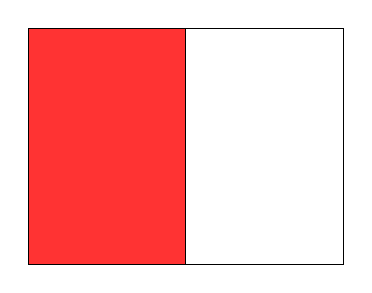
\begin{tikzpicture}
        \draw[fill=red!80] (0,0) -- (0,3) -- (2,3) -- (2,0) -- (0,0);
        \draw (2,3) -- (4,3) -- (4,0) -- (2,0) -- (2,3);
        \end{tikzpicture}}
\ffigbox{\caption{Flag ABA}\label{fig:flag-ABA}}
        {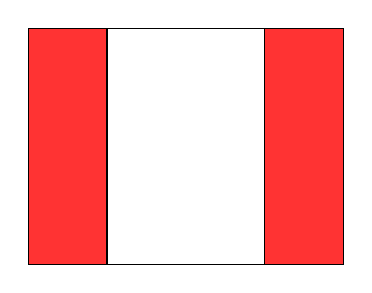
\begin{tikzpicture}
        \draw[fill=red!80] (0,0) -- (0,3) -- (1,3) -- (1,0) -- (0,0);
        \draw (1,3) -- (3,3) -- (3,0) -- (1,0) -- (1,3);
        \draw[fill=red!80] (3,3) -- (4,3) -- (4,0) -- (3,0) -- (3,3);
        \end{tikzpicture}}
\end{floatrow}
\end{figure}

As we saw in the previous sections, Polish encodes topological sensitivity lexically by differentiating between distinct partitive words. As in Polish, Brazilian Portuguese distinguishes between distinct half-words, namely \textit{metade} and \textit{meio} `half'. The former has nominal features and takes the partitive \textit{da}-phrase, whereas the latter is an adjectival expression agreeing with a modified noun in number and gender. Interestingly, similarly to Polish half-words \textit{metade} and \textit{meio} differ with respect to both their distributional and referential properties.\largerpage

Let us first consider the difference in the distribution of the two Brazilian Portuguese partitive expressions. While \textit{metade} patterns with \textit{połowa} in not being picky about the type of predicate within the \textit{da}-phrase it can combine with, see \ref{ex:distribution-metade}, \textit{meio} appears to correspond to \textit{pół} and \textit{połówka}. 

\ex. Brazilian Portuguese (Muriel Assmann, p.c.)\label{ex:distribution-metade}
\ag. metade da ma{\c{c}}{\~{a}}\label{ex:distribution-metade-sg}\\
half$_1$ the\textsc{.sg.f} apple\textsc{.f}\\
`half of the apple'
\bg. metade das ma{\c{c}}{\~{a}}s\label{ex:distribution-metade-pl}\\
half$_1$ the\textsc{.pl.f} apples\textsc{.f}\\
`half of the apples'
\bg. metade do suco\label{ex:distribution-metade-mass}\\
half$_1$ the\textsc{.sg.m} juice\textsc{.m}\\
`half of the juice'

As demonstrated in \ref{ex:distribution-meio-mass}, \textit{meio} cannot form a partitive with a mass term. Moreover, when combined with a plural noun it lacks a half-of-a-plurality reading, i.e., it cannot be interpreted as a quantifier over individuals making up the denoted plurality. Instead it can only operate on the subatomic level of particular members of the plurality denoted by a modified noun, i.e., it gets a half-of-a-singularity interpretation exclusively. In other words, \textit{meio} can only occur in an entity partitive and not in a set partitive. For instance, \ref{ex:distribution-meio-pl} cannot refer to a half of the total number of apples. The only interpretation available regards a plurality of apple halves.\largerpage

\ex. Brazilian Portuguese (Muriel Assmann, p.c.)\label{ex:distribution-meio}
\ag. meia ma{\c{c}}{\~{a}}\label{ex:distribution-meio-sg}\\
half$_{2}$\textsc{.sg.f} apple\textsc{.f}\\
`half of the apple'
\bg. meias ma{\c{c}}{\~{a}}s\label{ex:distribution-meio-pl}\\
half$_{2}$\textsc{.pl.f} apples\textsc{.f}\\
`apple halves'
\a. part-of-a-singularity reading
\b. \#part-of-a-plurality reading
\z. 
\bg. \#meio suco\label{ex:distribution-meio-mass}\\
half$_{2}$\textsc{.sg.m} juice\textsc{.m}\\
Intended: `half of the juice'

It seems plausible to posit that the contrasts between the phrases in \ref{ex:distribution-metade} and \ref{ex:distribution-meio} follow from topological restrictions imposed by \textit{meio} and \textit{metade} on what they select, analogously to the distinction between Polish \textit{pół} and \textit{połówka}, on the one hand, and \textit{połowa}, on the other. In other words, the nominal half-word \textit{metade} is topology-neutral, and thus can combine with DPs that denote integrated objects as well as those that have scattered entities in their extensions. On the other hand, adjectival \textit{meio} appears to be sensitive to the type of topological relations holding between parts of the referents of NPs it modifies. In particular, it requires integrated wholes. From a syntactic perspective, \textit{meio} as a nominal modifier sits lower in the structure than \textit{metade} which takes the whole DP as its complement. In other words, \textit{meio} is an adjective that is merged with the NP. Assuming that the NumP is higher than the AP \citep[e.g.,][]{ritter1991two,ritter1992cross}, this might explain scopal properties of \textit{meio} when it comes to subatomic quantification with respect to regular plurals, i.e., why \ref{ex:distribution-meio-pl} denotes a plurality of halves rather than half of a plurality. However, \textit{meio} can also combine with lexical plurals such as pluralia tantum, see \ref{ex:distribution-meio-pl.tant}, and it has been argued that the plural in lexical plurals is significantly lower, i.e., inside the \textit{n}P \citep[see, e.g.,][]{acquaviva2008lexical,alexiadou2011plural,smith2015feature,smith2017lexical}.\largerpage[2]

\ex. Brazilian Portuguese (Muriel Assmann, p.c.)
\bg.[] meio {\'{o}}culos\label{ex:distribution-meio-pl.tant}\\
half$_{2}$\textsc{.m} eye-glasses\textsc{.m}\\
`half of a pair of eye-glasses' or\\
`halves of eye-glasses'
\a. part-of-a-singularity reading
\b. \#part-of-a-plurality reading
\z.

Notice that \ref{ex:distribution-meio-pl.tant} gets a similar interpretation as the phrase in \ref{ex:distribution-meio-pl}, i.e., denotes a plurality of halves or rather, due to the number-neutrality of \textit{{\'{o}}culos} `eye-glasses', either a plurality of halves or one half of an object. I argue that this fact alongside the infelicity of phrases where \textit{meio} modifies mass terms, see \ref{ex:distribution-meio-mass}, supports the semantic explanation of the observed behavior in terms of topological sensitivity.

Even more interestingly, the results of the flag test show that \textit{meio} in fact patterns with Polish \textit{połówka}. As reported by my informant, the sentence with the proportional partitive with \textit{metade} in \ref{ex:flag-test-portuguese-metade} is true both in the flag AB scenario, see \figref{fig:flag-AB}, and in the flag ABA scenario, see \figref{fig:flag-ABA}. However, the sentence involving \ref{ex:flag-test-portuguese-meio} is judged true only in the former case and false in the latter. This means that \textit{metade} does not impose any topological restrictions on the portion of an entity denoted by the downstairs DP, wheres \textit{meio} yields only integrated parts.

		\ex. Brazilian Portuguese (Muriel Assmann, p.c.)\label{ex:flag-test-portuguese}
        \ag. Metade da bandeira é vermelha.\label{ex:flag-test-portuguese-metade}\\
		half$_1$ the flag is red\\
		`Half the flag is red.'
		\a. AB
		\b. ABA
		\z.
		\bg. Meia bandeira é vermelha.\label{ex:flag-test-portuguese-meio}\\
		half$_2$ flag is red\\
		`A half of the flag is red.'
		\a. AB
		\b. \#ABA
		\z.

A similar pattern is attested in Dutch where the distinction between the nominal expression \textit{helft} `half', on the one hand, see \ref{ex:flag-test-dutch-de-helft-van}, and adjectival \textit{half} `half', on the other, see \ref{ex:flag-test-dutch-halve}, is used in order to indicate the discussed contrast.\largerpage

\ex. Dutch (Erlinde Meertens, Izabela Jordanoska, p.c.)\label{ex:flag-test-dutch}
\ag. De helft van de vlag is rood.\label{ex:flag-test-dutch-de-helft-van}\\
		the half$_1$ of the flag is red\\
		`Half the flag is red.'
		\a. AB
		\b. ABA
		\z.
		\bg. De halve vlag is rood.\label{ex:flag-test-dutch-halve}\\
		the half$_2$ flag is red\\
		`A half of the flag is red.'
		\a. AB
		\b. \#ABA
		\z.

The half-word \textit{helft} forms a standard proportional entity partitive by combining with the prepositional \textit{van}-phrase which takes a singular DP as its complement (\citealt{de_hoop1997semantic,de_hoop2003partitivity}; see also \citealt[pp. 16--18]{cleven2013syntax}). On the other hand, Dutch \textit{half} resembles \textit{meio} in that it shows agreement with the modified NP. The suffix \textit{-e} on \textit{half} shows up when the noun is either definite or common gender, or both, as in the case of \ref{ex:flag-test-dutch-halve}, where it is spelled as \textit{halve}. As in the Brazilian Portuguese example, the flag test shows that \textit{helft} licenses both a continuous-half and a discontinuous-half interpretation, whereas adjectival \textit{half/halve} disallows the latter reading. In other words, while the sentence in \ref{ex:flag-test-dutch-de-helft-van} is reported to be true of both \figref{fig:flag-AB} and \ref{fig:flag-ABA}, \ref{ex:flag-test-dutch-halve} is judged false in the ABA flag scenario. This fact strongly suggests that Dutch lexicalized the distinction between topologically neutral and topologically sensitive partitive words. While \textit{helft} is similar to Polish \textit{połowa} or Brazilian Portuguese \textit{metade} in that it simply returns an entity constituting 50\% of a whole, truth conditions imposed by \textit{half/halve} are stronger, i.e., the partitive yields a half that needs to be integrated.  

It turns out that, as in Polish, Brazilian Portuguese and Dutch distinguish between topology-neutral and topology-sensitive half-words lexically. However, it is not the only way the distinction can be encoded in natural language. Thus, let us now consider a few strategies languages use to differentiate between the two partitive meanings in question that I identified in this chapter. Interestingly, different structures give rise to similar semantic effects concerning topological relations in subatomic quantification. The sample discussed here is relatively small, but the discussed data suggest that the observed semantic phenomenon is systematic and cross-linguistically valid. 

Let us start with the syntactic distinction occurring in English, as already mentioned in \ref{ex:half-an-half-of-english}. From a morphological point of view there is no contrast between the partitive word \textit{half} in \ref{ex:flag-test-english-half} and \ref{ex:flag-test-english-a-half-of}. Nevertheless, the syntactic structures in which it appears in each of the two sentences significantly differ (see \citealt{vannestal2004syntactic} for discussion). 
		
		\ex.\label{ex:flag-test-english} English (Jonathan Bobaljik, Jeffrey Parrott, p.c.)
        \a. Half the flag is red.\label{ex:flag-test-english-half}
		\a. AB
		\b. ABA
		\z.
		\b. A half of the flag is red.\label{ex:flag-test-english-a-half-of}
		\a. AB
		\b. \#ABA
		\z.

In \ref{ex:flag-test-english-half}, \textit{half} is a predeterminer since it can occur before regular determiners such as articles and demonstratives \citep[pp. 257--258]{quirk_greenbaum_leech_svartvik1985comprehensive}. On the other hand, in \ref{ex:flag-test-english-a-half-of} \textit{half} forms a standard proportional entity partitive by taking the \textit{of}-phrase with a singular DP as its complement. In this environment it seems to have nominal properties since it can be preceded by a determiner and it allows for numeral and adjectival modification \citep[p. 434]{huddleston_pullum2002cambridge}. The syntactic distinction translates into a semantic difference. Specifically, the sentence in \ref{ex:flag-test-english-half} is considered appropriate with respect to both the AB and ABA flag in \figref{fig:flag-AB} and \ref{fig:flag-ABA}, respectively, whereas \ref{ex:flag-test-english-a-half-of} would be judged true only in the first scenario.\footnote{A reviewer comments that they prefer \textit{one half of the flag} over \textit{a half of the flag} in this context. Though this raises an interesting question concerning interspeaker and/or dialectal variation, I ignore this issue here and simply report on my informants' judgments.} The contrast shows the relevance of topology in subatomic quantification even in the absence of distinct lexical items differentiating between a continuous-part and a discontinuous-part interpretation. In other words, it appears that natural language can employ purely syntactic means in order to indicate the notion of topological integrity of parts. Notice that the half-word in \ref{ex:flag-test-english-a-half-of} is preceded by the article. Superficially, the distinction between \textit{half} and \textit{a half of} resembles to some extent the contrast between the \textit{part}-expressions \textit{part of} and \textit{a part of}. The appearance of the indefinite article suggests that the latter should be treated on a par with count nominals and countability seems to imply spatial integrity.\largerpage

Another strategy is employed in German. At first blush, it might appear to pattern with Brazilian Portuguese and Dutch since it also distinguishes between the nominal half-word \textit{Hälfte} `half' and adjectival \textit{halb} `half'. However, German half-words display non-trivial interactions with determiners. While \textit{Hälfte} with the definite article \textit{die} shows similar behavior with respect to count singulars, plurals, and mass terms as Brazilian Portuguese \textit{metade}, see \ref{ex:distribution-halfte-def}, it is infelicitous with mass nouns when preceded by indefinite \textit{eine}, see \ref{ex:distribution-halfte}. 

\ex. German (Berit Gehrke, p.c.)\label{ex:distribution-halfte-def}
\ag. die Hälfte des Apfels\label{ex:distribution-halfte-sg-def}\\
the half$_1$ the\textsc{.gen} apple\textsc{.gen} \\
`half of the apple'
\bg. die Hälfte der Äpfel\label{ex:distribution-halfte-pl-def}\\
the half$_1$ the\textsc{.gen}  apples\textsc{.gen} \\
`half of the apples'
\bg. die Hälfte des Saftes\label{ex:distribution-halfte-mass-def}\\
the half$_1$ the\textsc{.gen}  juice\textsc{.gen} \\
`half of the juice'

\ex. German (Berit Gehrke, p.c.)\label{ex:distribution-halfte}
\ag. eine Hälfte des Apfels\label{ex:distribution-halfte-sg}\\
a half$_1$ the\textsc{.gen} apple\textsc{.gen} \\
`a half of the apple'
\bg. eine Hälfte der Äpfel\label{ex:distribution-halfte-pl}\\
a half$_1$ the\textsc{.gen}  apples\textsc{.gen} \\
`half of the apples'
\bg. \#eine Hälfte des Saftes\label{ex:distribution-halfte-mass}\\
a half$_1$ the\textsc{.gen}  juice\textsc{.gen} \\
Intended: `half of the juice'

On the other hand, definite DPs with adjectival \textit{halb} differ from Brazilian Portuguese phrases with \textit{meio} in that they can combine felicitously with all the types of expressions in question including mass nouns, see \ref{ex:distribution-halb-definite}. However, when preceded by the definite article, \textit{halb} is odd with mass nouns, and thus patterns with \textit{meio}, see \ref{ex:distribution-halb}.\largerpage

\ex. German (Nina Haslinger, p.c.)\label{ex:distribution-halb-definite}
\ag. der halbe Apfel\label{ex:distribution-halb-definite-sg}\\
the\textsc{.sg.m} half$_{2}$\textsc{.sg.m} apple\textsc{.m}\\
`the apple half'
\bg. die halben Äpfel\label{ex:distribution-halb-definite-pl}\\
the\textsc{.pl} half$_{2}$\textsc{.pl} apples\\
`the apple halves'
\a. part-of-a-singularity reading
\b. \#part-of-a-plurality reading
\z.
\bg. der halbe Saft\label{ex:distribution-halb-definite-mass}\\
the\textsc{.sg.m} half$_{2}$\textsc{.sg.m} juice\textsc{.m}\\
`half of the juice'

\ex. German (Nina Haslinger, p.c.)\label{ex:distribution-halb}
\ag. ein halber Apfel\label{ex:distribution-halb-sg}\\
a\textsc{.sg.m}  half$_{2}$\textsc{.sg.m} apple\textsc{.m}\\
`apple half'
\bg. halbe Äpfel\label{ex:distribution-halb-pl}\\
half$_{2}$\textsc{.pl}  apples\\
`apple halves'
\a. part-of-a-singularity reading
\b. \#part-of-a-plurality reading
\z.
\bg. \#halber Saft\label{ex:distribution-halb-mass}\\
half$_{2}$\textsc{.sg.m} juice\textsc{.m} \\
Intended: `half of the juice'

In addition, the examples with the definite article in \ref{ex:distribution-halb-definite} seem to also have an additional expressive intensifier reading of the sort `all those apples'. For instance, it would be appropriate when half of the apples were splattered across the street and the speaker were expressive about this situation (somewhat like \textit{totally}).\footnote{I would like to thank Berit Gehrke for sharing this observation with me.}\largerpage

The facts discussed above suggest that whether \textit{Hälfte} and \textit{halb} are sensitive to the spatial constitution of referents of the NP they attach to depends on the determiner. In particular, their selectional restrictions suggest that German definite DPs with half-words are topology-neutral, whereas their indefinite counterparts are topology-sensitive. The results of the flag test seem to support that idea. As witnessed in \ref{ex:flag-test-german-halfte} and \ref{ex:flag-test-german-halb}, sentences with definite DPs involving \textit{Hälfte} and \textit{halb} are judged true in both the AB and the ABA flag scenario. Unlike in the case of Brazilian Portuguese \textit{meio}, there is no contrast between \textit{Hälfte} and the expressive reading of \textit{halb} with respect to the the spatial make up of the partial entity they yield here.\footnote{Note, however, that \ref{ex:flag-test-german-halb} has also a strongly individuating reading that there is one piece of cloth, which is half a flag (the other half is ripped off), and that half-flag is red.}

\ex. German (Berit Gehrke, Nina Haslinger, Maximilan Prüller, p.c.)\label{ex:flag-test-german}
\ag. Die Hälfte der Fahne ist rot.\label{ex:flag-test-german-halfte}\\
		the half$_1$ the\textsc{.gen} flag is red\\
		`Half the flag is red.'
		\a. AB
		\b. ABA
		\z.
		\bg. Die halbe Fahne ist rot.\label{ex:flag-test-german-halb}\\
		the half$_2$ flag is red\\
		`Half the flag is red.'
		\a. AB
		\b. ABA
		\z.

Now, consider the indefinite counterparts of \ref{ex:flag-test-german} in \ref{ex:flag-test-german-indef}. Both \ref{ex:flag-test-german-halfte-indef} and \ref{ex:flag-test-german-halb-indef} display the kind of semantic behavior observed in typologically sensitive expressions such as Polish \textit{połówka}, Brazilian Portuguese \textit{meio}, and Dutch \textit{half}, i.e., they would be true only if a continuous part of the flag were red.\footnote{Again, the non-expressive reading of \ref{ex:flag-test-german-halb-indef} is that there is a half of the flag that is cut off or separated from the rest.} This shows that the source of topological sensitivity is the interaction between the half-word and the determiner rather than that it is encoded lexically.  

\ex. German (Berit Gehrke, p.c.)\label{ex:flag-test-german-indef}
\ag. Eine Hälfte der Fahne ist rot.\label{ex:flag-test-german-halfte-indef}\\
a half$_1$ the\textsc{.gen} flag is red\\
`A/One half of the flag is red.'
		\a. AB
		\b. \#ABA
		\z.
\bg. Eine halbe Fahne ist rot.\label{ex:flag-test-german-halb-indef}\\
a half$_2$  flag is red\\
`One piece, which is half a flag, is red.'
		\a. AB
		\b. \#ABA
		\z.

Furthermore, there is yet another topology-sensitive construction in German. In particular, consider the subject of the sentence in \ref{ex:german-eine-halfte-definite-article} involving the half-word \textit{Hälfte} preceded by both what at first blush appears to be an indefinite article and the definite article \textit{die}. Notice, however, that \textit{eine} in this environment is not an indefinite article, but rather the numeral `one'. The mere fact that it can combine with the definite article \textit{die} suggests that it is an expression of a different type. Furthermore, unlike regular indefinite articles, it is always stressed. As shown by the ungrammaticality of \ref{ex:german-halfte-stress}, in this construction one cannot put stress on the half-word.\largerpage

\ex. German (Berit Gehrke, Maximilian Prüller, p.c.)\label{ex:german-eine-halfte}
\ag. Die EINE Hälfte der Fahne ist rot.\label{ex:german-eine-halfte-definite-article}\\
the one half$_1$ the\textsc{.gen} flag is red.\\
`The half of the flag is red.'
\bg. *Die eine HÄLFTE der Fahne ist rot.\label{ex:german-halfte-stress}\\
the a half$_1$ the\textsc{.gen} flag is red.\\
Intended: `The half of the flag is red.'

The truth conditions of sentences with the \textit{die eine Hälfte} partitive expression contrast with the truth conditions of the sentences involving definite proportional partitives examined so far. For instance, consider \ref{ex:flag-test-german2}.  

\ex. German (Berit Gehrke, Nina Haslinger, Maximilan Prüller, p.c.)\label{ex:flag-test-german2}
\ag. Die Hälfte der Fahne ist rot.\label{ex:flag-test-german-die-halfte}\\
		the half$_1$ the.\textsc{gen} flag is red\\
		`Half the flag is red.'
		\a. AB
		\b. ABA
		\z.
		\bg. Die eine Hälfte der Fahne ist rot.\label{ex:flag-test-german-die-eine-halfte}\\
		the a/one half$_1$ the\textsc{.gen} flag is red\\
		`One half of the flag is red.'
		\a. AB
		\b. \#ABA
		\z.

As we have already discussed, \ref{ex:flag-test-german-die-halfte} is true of both relevant scenarios, i.e.,  \figref{fig:flag-AB} and \ref{fig:flag-ABA}. However, \ref{ex:flag-test-german-die-eine-halfte} is consistently judged false in the flag ABA situation. This shows that German developed a rather complex system in which the semantic distinction between different proportional partitive expressions, i.e., topologically neutral partitives, on the one hand, and topology-sensitive expressions, on the other, results from the interaction between the half-word, definiteness, and the numeral. The expressions are distinguished from each other both lexically and structurally with the most marked form being at the same time  semantically most complex.

Finally, the examined contrast involving yet another two types of constructions is found in Mandarin. The two structures are provided in \ref{ex:flag-test-mandarin}. 

		\ex. Mandarin (Chang Liu, p.c.)\label{ex:flag-test-mandarin}
        \ag. gu{\'{o}} q{\'{i}} de y{\'{i}}-b{\`{a}}n sh{\`{i}} h{\'{o}}ng de.\label{ex:flag-test-mandarin-yiban}\\
		national flag \textsc{lnk} one-half \textsc{cop} red \textsc{lnk}\\
		`Half the national flag is red.'
		\a. AB
		\b. ABA
		\z.
		\pagebreak\bg. b{\`{a}}n-mi{\`{a}}n gu{\'{o}} q{\'{i}} sh{\`{i}} h{\'{o}}ng de.\label{ex:flag-test-mandarin-banmian}\\
		half-\textsc{clf} national flag \textsc{cop} red \textsc{lnk}\\
		`A half of the national flag is red.'
		\a. AB
		\b. \#ABA
		\z.

In \ref{ex:flag-test-mandarin-yiban}, the partitive meaning is conveyed by the phrase involving the proportional expression \textit{y{\'{i}}-b{\`{a}}n} `half' related by the associative marker \textit{de} to the nominal \textit{gu{\'{o}} q{\'{i}}} `national flag' (\citealt[p. 294]{jing-schmidt2005dramatized}; \citealt{jin2018partition}). In this construction, the half-word \textit{b{\`{a}}n} does not follow a classifier and combines directly with the preceding cardinal numeral \textit{y{\'{i}}} `one' forming a constituent. It is possible that \textit{y{\'{i}}} in \textit{y{\'{i}}-b{\`{a}}n} is in fact a grammaticalized expression interpreted as an indefinite rather than a numeral (see \citealt[p. 127]{hsieh2008internal}; \citealt{jin2018partition}).\footnote{See also \citet[p. 46]{hsieh2008internal} and \citet{zhang2011constituency} for the discussion of issues regarding constituency and other types of environments \textit{b{\`{a}}n} appears in.} In any case, this structure is topologically neutral and yields both integrated and discontinuous halves of entities since sentences such as \ref{ex:flag-test-mandarin-yiban} are reported to be true of the flag in \figref{fig:flag-AB} as well as the one in \figref{fig:flag-ABA}. In \ref{ex:flag-test-mandarin-banmian}, however, the partitive morpheme \textit{b{\`{a}}n} behaves more like a quantifier since it needs to combine with the classifier \textit{mi{\`{a}}n} dedicated to counting flat and smooth objects such as mirrors in order to quantify over parts of the national flag denoted by the nominal. Therefore, it appears that in this case the syntactic status of the half-word is on a par with cardinals. And again, a different structure corresponds to a different semantics. Unlike \ref{ex:flag-test-mandarin-yiban}, the sentence in \ref{ex:flag-test-mandarin-banmian} can only mean that an integrated half of the national flag is red, i.e., it would be judged false in the scenario represented in \figref{fig:apple_discont-half}.

The Mandarin example discussed above concludes this brief exploration of cross-linguistic strategies of encoding sensitivity to topological notions in partitive expressions. Though the sample of languages examined here was relatively small and most probably more strategies await to be discovered within a future thorough cross-linguistic investigation, the presented evidence proves that natural language encodes subtle topological distinctions in the domain of partitivity. The contrasts examined here are often very slight but a careful examination suggests that the topology-related phenomena in question are not something idiosyncratic but rather occur systematically across languages.

In the next section, I will discuss yet another class of expressions that might shed new light on the issues related to the interplay of quantification and topology. In particular, I will consider some similarities and contrasts concerning two whole-adjectives in Polish, namely \textit{cały} `whole' and \textit{kompletny} `complete'. To this end, I will explore two different respects of being entire as well as the interaction between whole-adjectives and different types of nominals from the perspective of subatomic quantification and topological sensitivity.

\section{Whole-adjectives}\label{sec:whole-adjectives}

Due to contrasts parallel to the one illustrated in \ref{ex:whole-adjectives-ferret}, adjectives such as \textit{whole} and \textit{entire} have been analyzed as universal quantifiers over parts \citep{moltmann1997parts} or maximizing modifiers, i.e., expressions restricting exception tolerance \citep{morzycki2002wholes}.\footnote{\citet{morzycki2002wholes} builds on \citeposst{brisson1998distributivity} analysis of \textit{all} in terms of maximizing modification.} There is a strong intuition that compared to \ref{ex:ferret} the sentence in \ref{ex:whole-ferret} implies that no part of the entity in question is exempt from having to satisfy the main predicate. In particular, \ref{ex:ferret} would be true if a sufficiently significant proportion of the ferret were under the water, i.e., if part of a paw or a tail were not submerged, under most circumstances the sentence would not be considered false. However, the proposition expressed by \ref{ex:whole-ferret} is stronger. It states that all the parts of the ferret are submerged.

\ex. English (\citealt{morzycki2002wholes}; adapted)\label{ex:whole-adjectives-ferret}
\a. The ferret is submerged.\label{ex:ferret}
\b. The \{whole/entire\} ferret is submerged.\label{ex:whole-ferret}

In Polish, alongside the standard whole-adjective \textit{cały} `whole', there is yet another expression that shares some of its semantic properties yet differs in an interesting respect, namely the adjective \textit{kompletny} `complete'. Though there is a partial overlap between the two expressions in question in terms of their distribution, they show quite different patterns. 

Let us first consider the distributional potential of the whole-adjective \textit{cały}. What is interesting about this expression is that it can be used for universal quantification over parts of stuff denoted both by singular count nouns and mass terms. Specifically, \ref{ex:distribution-caly-sg} refers to all the material parts making up a particular apple, whereas \ref{ex:distribution-caly-mass} is true of an entity comprising all the quantities of juice in a relevant context, i.e., the total amount of juice. Interestingly, when modifying a plural expression such as \ref{ex:distribution-caly-pl}, in some contexts \textit{cały} can scope over the plural. In other words, \ref{ex:distribution-caly-pl} is true of a plurality of whole apples but it can also be true of a whole plurality of not necessarily whole apples.\largerpage[-1]\pagebreak

		\ex. Polish\label{ex:distribution-caly}
        \ag. całe jabłko\label{ex:distribution-caly-sg}\\
		whole\textsc{.sg.n} apple\textsc{.n}\\
		`whole apple' or\\`all (of) the apple'
        \bg. cały sok\label{ex:distribution-caly-mass}\\
		whole\textsc{.sg.m} juice\textsc{.m}\\
		`all (of) the juice'
		\bg. całe jabłka\label{ex:distribution-caly-pl}\\
		whole\textsc{.pl} apples\\
		`whole apples' or\\`all (of) the apples'
        \a. plural > whole
        \b. whole > plural
        \z.

Admittedly, the cases in which \textit{cały} can outscope the plural are restricted and in many environments such a reading is either unavailable or marked. However, there are contexts in which it is definitely possible. One such example is illustrated by the sentence in \ref{ex:caly-scope}.

\ex. Polish (Adam Przepiórkowski, p.c.)\label{ex:caly-scope}
\bg.[] Szczury zjadły całe jabłka, choć większość {i tak} była już wcześniej nadgryziona przez myszy.\\
rats ate whole\textsc{.acc} apples\textsc{.acc} though most anyway was already earlier nibbled by mice\textsc{.acc}\\
`Rats ate all of the apples, although most of them were already nibbled off by mice.'
		
Compared to \textit{cały}, the distribution of \textit{kompletny} is significantly restricted. Intuitively, this is due to the fact that it seems to presuppose a certain complexity in terms of a part-whole structure. In particular, it can only modify nominals referring to objects consisting of multiple easily recognizable and distinguishable parts such as utensils and clothes.\footnote{There is yet another meaning of \textit{kompletny} that could be glossed as `total' which does not impose such a constraint. This use is especially frequent in colloquial Polish; however, it will not be considered here.} 

In addition to this restriction, the whole-adjective \textit{kompletny} differs from \textit{cały} in that it can never scope over the plural. For instance, due to the fact that computers consist of many detachable elements, \ref{ex:distribution-kompletny-sg} is a meaningful phrase in Polish. Similarly, when combined with an object mass term it implies that all discrete objects comprising the extension of the noun are in place. For example, \ref{ex:distribution-kompletny-mass} would be true of a collection of equipment where there is no item missing. Moreover, \textit{kompletny} frequently appears with collective nouns such as \textit{zestaw} `set' and \textit{kolekcja} `collection', which denote groups of artifacts. On the other hand, when modifying a plural expression, as in \ref{ex:distribution-kompletny-pl}, \textit{kompletny} cannot assert the denoted property of a plurality as such, but rather of singular individuals. In other words, \ref{ex:distribution-kompletny-pl} means that individual computers are complete and not the plurality thereof.

		\ex. Polish\label{ex:distribution-kompletny}
        \ag. kompletny komputer\label{ex:distribution-kompletny-sg}\\
		complete\textsc{.sg.m} computer\textsc{.m}\\
		`complete computer'
        \bg. kompletny sprzęt\label{ex:distribution-kompletny-mass}\\
		complete\textsc{.sg.m} equipment\textsc{.m}\\
        `complete equipment'
		\bg. kompletne komputery\label{ex:distribution-kompletny-pl}\\
		complete\textsc{.pl} computers\\
		`complete computers'
        \a. plural > complete
        \b. \#complete > plural
        \z.

Notice also that both \textit{cały} and \textit{kompletny} can combine with pluralia tantum, see \ref{ex:caly-pl.tant}--\ref{ex:kompletny-pl.tant}. The plurale tantum nominal \textit{nożyczki laparaskopowe} `laparoscopic graspers' denotes a specialized object consisting of multiple detachable and replaceable elements, which makes it a proper expression to be modified by \textit{kompletny}. In both cases, the whole phrase is ambiguous between a singular and a plural reading, i.e., it either refers to one whole or complete object, respectively, or to a plurality of whole or complete objects. 

\ex. Polish\label{ex:calykompletny-pl.tant}
\ag. całe nożyczki laparoskopowe\label{ex:caly-pl.tant}\\
whole\textsc{.pl} scissors laparoscopic\textsc{.pl}\\
`whole laparoscopic graspers' or\\
`all of the laparoscopic graspers'
\bg. kompletne nożyczki laparoskopowe\label{ex:kompletny-pl.tant}\\
complete\textsc{.pl} scissors laparoscopic\textsc{.pl}\\
`complete laparoscopic graspers'

The reading on which the whole-adjective would impose a semantic restriction on a plurality can be available only for \ref{ex:caly-pl.tant}, i.e., only this phrase can mean something like a whole plurality of laparoscopic graspers. This can be observed in a shopping context, where a sentence such as \ref{ex:caly-pl.tant-scope} means that the owners of the store ran out of laparoscopic gaspers. Given the fact that the plural in plurale tantum nouns was argued to be inside the \textit{n}P \citep[see, e.g.,][]{acquaviva2008lexical,alexiadou2011plural,smith2015feature,smith2017lexical}, data like \ref{ex:caly-pl.tant-scope} suggest that \textit{cały} can enter into a scopal relation with a plurality even when it is encoded very low in the structure.

\ex. Polish\label{ex:caly-pl.tant-scope}
\bg.[] Dziś było tyle zamówień ze szpitali, że sprzedaliśmy całe nożyczki laparoskopowe.\\
today was so.many orders\textsc{.gen} from hospitals\textsc{.gen} that we.sold whole\textsc{.pl} scissors laparoscopic\textsc{.pl}\\
`Today there were so many orders from hospitals that we sold out all laparoscopic graspers.' 

\tabref{tab:distribution-of-polish-whole-adjectives} gives an overview of the distribution of the Polish whole-adjectives \textit{cały} and \textit{kompletny} as discussed above. While both can co-occur with singular count nouns and mass terms, the latter requires the modified noun to refer to complex entities consisting of multiple easily individuated parts. On the other hand, when combined with regular plurals, only \textit{cały} can scope over the plural. In other words, what is targeted by \textit{kompletny} is always the part-whole structure of a particular singular individual, whereas \textit{cały} in some cases can trigger universal quantification over singular objects making up a plural entity. 

		\begin{table}[h]
			\centering
			\begin{tabular}{lcccccc}
				\lsptoprule
				& \textsc{singulars} & \textsc{mass nouns}   & \textsc{plurals} \\ \midrule
				cały & $\checked$  & $\checked$    & $\checked$            \\ 
				kompletny & $\checked$    &  $\checked$    & \#            \\
				\lspbottomrule
			\end{tabular}
			\caption{Distribution of Polish \textit{whole} adjectives}
            \label{tab:distribution-of-polish-whole-adjectives}
		\end{table}

The evidence regarding the distribution of the Polish whole-adjectives in question suggests the distinction between integrated objects as prototypically denoted by singular count nouns and scattered entities designated by mass terms, on the one hand, and arbitrary sums of individuals referred to plural expressions, on the other. To some extent this contrast resembles what was observed with respect to the distribution of the piece-word \textit{kawałek} in \sectref{sec:piece-words} and \sectref{sec:mass-parts-quantitifes-and-pieces}. Before I move on to discussing some semantic differences between \textit{cały} and \textit{kompletny}, let us briefly examine a cross-linguistic context which might shed more light on the pattern observed in Polish. In the next section, I will consider data concerning a German whole-adjective modifying plural nouns.

\subsection{German \textit{ganz} and plurals}\label{sec:german-ganz-and-plurals}

As in Polish, in German the whole-adjective \textit{ganz} `whole' can be used as a universal quantifier over parts of matter making up referents of both singular count nouns as well as mass terms, as demonstrated in \ref{ex:distribution-ganz-sg}--\ref{ex:distribution-ganz-mass} \citep[see also][pp. 123--127]{moltmann1997parts}.

\ex. German (Nina Haslinger, p.c.)\label{ex:distribution-ganz}
        \ag. der ganze Apfel\label{ex:distribution-ganz-sg}\\
		the\textsc{.sg.m} whole\textsc{.sg} Apfel\textsc{.m}\\
		`the whole apple' or\\`all (of) the apple'
        \bg. der ganze Saft\label{ex:distribution-ganz-mass}\\
		the\textsc{.sg.m} whole\textsc{.sg} juice\textsc{.m}\\
        `all (of) the juice'

In addition, it has also been reported that at least in some German dialects the adjective \textit{ganz} `whole' gives rise to a universal quantification interpretation when modifying plural DPs (\citealt[pp. 123--127]{moltmann1997parts}; see also \citealt{igel-toappear-part}). This is claimed to be possible with plurals referring to sums constituting natural \linebreak wholes, i.e., sums whose members are considered as having less individuality, and thus do not appear to be prominent with respect to the whole \citep[p. 125]{moltmann1997parts}. For instance, consider \ref{ex:german-ganz}. 

\ex. German \citep[p. 125; adapted]{moltmann1997parts}\label{ex:german-ganz}
\ag. Die ganzen Kinder sind gekommen.\label{ex:german-ganz-children}\\
the\textsc{.pl} whole\textsc{.pl} children are come\\
`All the children have come.'
\bg. Die ganzen Bienen haben Maria gestochen.\label{ex:german-ganz-bees}\\
the\textsc{.pl} whole\textsc{.pl} bees have Maria stung\\
`All the bees have stung Maria.'

In the sentence in \ref{ex:german-ganz-children}, children are part of a more or less anonymous group, whereas in \ref{ex:german-ganz-bees} bees are perceived as constituents of a swarm. In both cases, the modifier \textit{ganz} seemingly quantifies over individuals making up the pluralities and the whole DP yields the total number of children and bees involved in coming and stinging, respectively.

However, under more rigorous investigation it appears that at least in one Austrian dialect showing the discussed behavior there is an important distinction between \textit{ganz} and the universal quantifier \textit{alle} `all'. Whatever the exact semantic contribution of \textit{ganz}, it seems that unlike \textit{alle} it allows for exceptions. For instance, consider the contrast given in \ref{ex:german-ganz-alle-exceptions}. While the sentence in \ref{ex:german-ganz-exceptions} can be supplemented with another clause stating that not all of the children have come, \ref{ex:german-alle-exceptions} obviously excludes such a continuation.\footnote{In \ref{ex:german-ganz-alle-exceptions}, I ignored dialectal phonological features and simply provided Standard German spelling.}

\ex. Viennese German (Maximilian Prüller, p.c.)\label{ex:german-ganz-alle-exceptions}\\
\textit{Scenario}: My neighbors have 10 children and I don't like them but have to invite them.
\ag. Dann sind die Nachbarn mit ihren ganzen Kindern gekommen. Zwei waren krank zuhause, und es waren {immer noch} acht!\label{ex:german-ganz-exceptions}\\
then are the neighbors with their\textsc{.dat} whole\textsc{.dat.pl} children\textsc{.dat} come two were ill at.home and it were still eight\\
`Then the neighbors have come with their children. Two of them were ill and stayed home, but there were still eight!'
\bg. \# Dann sind die Nachbarn mit allen ihren Kindern gekommen. Zwei waren krank zuhause, und es waren {immer noch} acht!\label{ex:german-alle-exceptions}\\
then are the neighbors with all\textsc{.dat} their\textsc{.dat} children\textsc{.dat} come two were ill at.home and it were still eight\\
Intended: `Then the neighbors have come with all their children. Two of them were ill and stayed home, but there were still eight!'

Although definitely more systematic research is required to establish what exactly the properties of \textit{ganz} are, I take the data in \ref{ex:german-ganz} as evidence suggesting that German \textit{ganz} patterns in the relevant respect with Polish \textit{cały}. In the next section, I will return to the alternation between \textit{cały} and \textit{kompletny} and examine two different aspects of wholeness.

\subsection{Integrity vs. maximality}\label{sec:integrity-vs-maximality}

There is yet another difference between the Polish whole-adjectives \textit{cały} and \textit{kompletny}, which also intuitively appears to be the most significant one. The difference relates to the distinction between two aspects of wholeness, which I will call an integrity component and a maximality component. The former is topological in nature and indicates that the parts of a whole are connected in such a way that they form an intact integrated object.\footnote{See also \citep[p. 127]{moltmann1997parts} for a remark on the integrity reading of German \textit{ganz} in predicate position as, e.g., in \ref{ex:german-ganz-integrity}.

\ex. German \citep[p. 127; adapted]{moltmann1997parts}\label{ex:german-ganz-integrity}
\bg.[] Das Glas ist noch ganz.\\
the glass is still whole\\
`The glass is still intact.'

} The latter, on the other hand, simply employs universal quantification over parts or mereological exhaustivity, and thus indicates that no part of a whole is missing.\footnote{However, see \citet{morzycki2002wholes} for arguments against treating whole-adjectives as universal quantifiers over parts based on the anaphoric and scope properties they give rise to. Instead, he proposes to treat them as maximizing modifiers. Since the main point here concerns the distinction between quantification over wholes and subatomic quantification, I only signal the problem here and leave it unaddressed.} 

Under ordinary circumstances these two aspects of wholeness are interrelated. Hence, the contrast between the two meanings might seem somewhat subtle and in many contexts it is probably difficult to detect. However, it is relatively easy to come up with examples where it becomes significant. For instance, consider the scenario described in \ref{ex:aspects-wholeness-caly}. 

\ex. Polish\\
\textit{Scenario}: Jan bought his daughter Marysia a model aircraft. After Marysia unwrapped the gift and opened the box, her brother Piotruś asks:\label{ex:aspects-wholeness-caly}
\ag. Czy ten samolot jest cały?\label{ex:aspects-wholeness-caly-int}\\
\textsc{int} this model.aircraft is whole\\
`Is this model aircraft whole?'
\bg. Nie, brakuje śmigła.\label{ex:aspects-wholeness-caly-exhaustive}\\
no it.lacks propeller\textsc{.gen}\\
`No, it lacks the propeller.'
\bg. Nie, trzeba go złożyć.\label{ex:aspects-wholeness-caly-integrity}\\
no, it.needs it\textsc{.acc} assemble\\
`No, it needs to be assembled.'

Notice that there are two kinds of model aircraft Jan might have bought for Marysia, namely either a pre-built model that has already been put together or a construction kit with a collection of separate parts that require gluing. Then, depending on whether Marysia got the former or the latter, her brother Piotruś's question in \ref{ex:aspects-wholeness-caly-int} can be understood along the lines of topological integrity or mereological exhaustivity. In particular, \ref{ex:aspects-wholeness-caly-exhaustive} provides an answer to a question implying a maximality reading, i.e., whether no part is missing, whereas \ref{ex:aspects-wholeness-caly-integrity} is a reply in terms of an integrity interpretation, i.e., whether the parts are connected. This shows that though the two ways in which being a whole can be understood are frequently related, they are in fact separate semantic phenomena and in some contexts only one of them can become prominent if not the only relevant aspect.

Now, let us compare what was observed in \ref{ex:aspects-wholeness-caly} with what happens in the same context when the question in \ref{ex:aspects-wholeness-kompletny-int} is slightly modified. Specifically, instead of \textit{cały} what appears in predicate position is the whole-adjective \textit{kompletny}. 

\ex. Polish\\
\textit{Scenario}: Jan bought his daughter Marysia a model aircraft. After Marysia unwrapped the gift and opened the box, her brother Piotruś asks:\label{ex:aspects-wholeness-kompletny}
\ag. Czy ten samolot jest kompletny?\label{ex:aspects-wholeness-kompletny-int}\\
\textsc{int} this model.aircraft is complete\\
`Is this model aircraft complete?'
\bg. Nie, brakuje śmigła.\label{ex:aspects-wholeness-kompletny-exhaustive}\\
no it.lacks propeller\textsc{.gen}\\
`No, it lacks the propeller.'
\bg. \#Nie, trzeba go złożyć.\label{ex:aspects-wholeness-kompletny-integrity}\\
no, it.needs it\textsc{.acc} assemble\\
`No, it needs to be assembled.'

Here, the only meaningful answer is the one in \ref{ex:aspects-wholeness-kompletny-exhaustive}. The reply in \ref{ex:aspects-wholeness-kompletny-integrity} is just remarkably odd. That is because \textit{kompletny}, unlike \textit{cały}, lacks the semantic component invoking integrity and implies exclusively the maximality aspect of wholeness. Therefore, the question in \ref{ex:aspects-wholeness-kompletny-int} can only be interpreted as whether the box includes all the relevant parts of the model aircraft. 

The contrast between the number of possible answers in \ref{ex:aspects-wholeness-caly} and \ref{ex:aspects-wholeness-kompletny} shows that \textit{cały} has two meaning components which correspond to maximality, on the one hand, and integrity, on the other. In contrast, \textit{kompletny} can be interpreted exclusively in terms of maximality. Importantly, however, it is not the case that \textit{cały} is ambiguous between two different readings. Rather, both aspects of wholeness need to be present. The reason is that in the context of \ref{ex:aspects-wholeness-caly-ambiguity} neither of the answers to the question in \ref{ex:aspects-wholeness-caly-ambiguity-int} makes much sense. If \textit{cały} were ambiguous, both \ref{ex:aspects-wholeness-caly-ambiguity-1} and \ref{ex:aspects-wholeness-caly-ambiguity-2} would be legitimate.

\ex. Polish (Adam Przepiórkowski, p.c.)\\
\textit{Scenario}: Jan bought his daughter Marysia a model aircraft. After Marysia unwrapped the gift and opened the box, her brother Piotruś asks:\label{ex:aspects-wholeness-caly-ambiguity}
\ag. Czy ten samolot jest cały?\label{ex:aspects-wholeness-caly-ambiguity-int}\\
\textsc{int} this model.aircraft is whole\\
`Is this model aircraft whole?'
\bg. \#Tak, jest cały, tylko trzeba go złożyć.\\
yes is whole only needs it\textsc{.acc} assemble\\
`Yes, it is whole, but it needs to be assembled.'\label{ex:aspects-wholeness-caly-ambiguity-1}
\bg. \#Tak, jest cały, tylko brakuje mu śmigła.\\
yes is whole only lacks it\textsc{.dat} propeller\textsc{.gen}\\
`Yes, it is whole, it only lacks the propeller.'\label{ex:aspects-wholeness-caly-ambiguity-2}

Though the distinction discussed in this section is subtle, it is systematic and can be detected in multiple environments. Even out of the blue the intuitions regarding the contrast between the sentence in \ref{ex:caly-interpretation} and \ref{ex:kompletny-interpretation} are very clear. The former states that all the relevant parts of the toy are in place or that the parts are connected, or most probably both, whereas the latter implies only that no relevant part of the toy is missing.\footnote{It is possible that the semantics of \textit{cały} is even stronger. As suggested by Adam Przepiórkowski (p.c.), in some contexts it seems to require that the object in question is not only maximal in the mereological sense and integrated in the topological sense, but also undamaged. Such a requirement seems to invoke a stronger topological notion, perhaps the notion of homeomorphism in the sense that, e.g., a broken sphere is not homeomorphic with an unbroken sphere. Though this is definitely a very interesting idea, I will leave careful investigation of its implications for future research.}\largerpage
		
		\ex. Polish\label{ex:caly-kompletny-interpretation}
        \ag. Ta zabawka jest cała.\label{ex:caly-interpretation}\\
		this toy is whole\\
		`This toy is whole.'
		\a. maximality meaning
		\b. integrity meaning
		\z.
		\bg. Ta zabawka jest kompletna.\label{ex:kompletny-interpretation}\\
		this toy is complete\\
		`This toy is complete.'
		\a. maximality meaning
		\b. \#integrity meaning
        \z.

\tabref{tab:interpretations-of-polish-whole-adjectives} recapitulates the findings. Distinguishing between the maximality and the integrity meaning component of wholeness allows us to conclude that while the Polish whole-adjective \textit{kompletny} is topology-neutral, \textit{cały} is not.  

		\begin{table}[h]
			\centering
			\begin{tabular}{lcccc}
				\lsptoprule
				& \textsc{maximality} & \textsc{integrity} \\ \midrule
				cały  & $\checked$    & $\checked$  \\
				kompletny & $\checked$   & * \\ \lspbottomrule
			\end{tabular}
			\caption{Interpretations of Polish whole-adjectives}
            \label{tab:interpretations-of-polish-whole-adjectives}
		\end{table}

The contrast concerning possible interpretations of the Polish whole-ad\-jec\-tives discussed in this section provides yet another piece of evidence that some natural language expressions are sensitive to topological relations holding between particular entities. Specifically, the whole-adjective \textit{cały} can be used to imply that all the parts of an object remain in such a spatial configuration that the object in question constitutes an integrated whole. In the next section, I will focus on the maximality aspect of wholeness. In particular, assuming that the semantics of \textit{cały} involves universal quantification over entities of some sort I will examine what exactly can constitute the domain of such quantification.

\subsection{Universal quantification over parts and wholes}\label{sec:universal-quantification-over-parts-and-wholes}

Though the Polish whole-adjective \textit{cały} can combine with a wide range of expressions including singular count nouns, prototypical mass terms, granulars, object mass nouns, and plurals, in each case the interpretation of the whole NP depends on the structure of the denotation of the modified noun. The difference becomes apparent when we distinguish between subatomic quantification, i.e., quantification over material parts making up building blocks of the denotation of a certain noun, and what, for the lack of a better term, I will call non-subatomic quantification, i.e., quantification above the subatomic level. Specifically, non-subatomic quantification covers both atomic quantification, i.e., quantification over singular individuals constituting pluralities of objects, as well as quantification over portions of substances as long as it does not target the internal structure of minimal building blocks of mass denotations, assuming there are any.\footnote{Though for a long time it was commonly assumed that there are no minimal building blocks in the denotations of mass nouns \citep[e.g.,][]{ter_meulen1980substances,link1983logical,bunt1985mass,landman1991structures}, some theories postulate that the denotations of mass nouns do in fact consist of minimal building blocks but these building blocks are in some way inaccessible for counting \citep[e.g.,][]{chierchia1998plurality,chierchia2010mass}. For an overview, see \citet{landman2011count}.} 

To illustrate the distinction, let us first consider the interpretative contrast between singular count nouns and liquid terms. For instance, the phrase in \ref{ex:quantification-caly-sg} involves subatomic quantification, whereas \ref{ex:quantification-caly-mass} does not. 

		\ex. Polish\label{ex:quantification-caly-sg-mass}
        \ag. całe jabłko\label{ex:quantification-caly-sg}\\
		whole\textsc{.sg.n} apple\textsc{.n}\\
		`whole apple' or\\
		`all (of) the apple'
		\a. subatomic quantification
		\b. \#non-subatomic quantification
        \z.
		\bg. cała woda\label{ex:quantification-caly-mass}\\
		whole\textsc{.sg.f} water\textsc{.f}\\
		`all (of) the water'
		\a. \#subatomic quantification
		\b. non-subatomic quantification
		\z.

The whole-adjective \textit{cały} in \ref{ex:quantification-caly-sg} quantifies universally over material parts of a single apple rather than, e.g., over individual apples making up a collection of apples. In other words, \ref{ex:quantification-caly-sg} does not mean something like `all apples' when the set of relevant apples consists of one object. On the other hand, in \ref{ex:quantification-caly-mass} \textit{cały} triggers universal quantification over entities in the extension of the modified mass noun, but it is impossible to interpret the phrase as meaning that some quantity of individual drops or molecules of water are whole. Rather, \ref{ex:quantification-caly-mass} designates the entire amount of the water in question. In addition, unlike \ref{ex:quantification-caly-sg}, the phrase in \ref{ex:quantification-caly-mass} does not imply the sense of integrity. The translations of the sentences in \ref{ex:quantification-caly-sg-subatomic} illustrate the difference.\largerpage[-1]

\ex. Polish\label{ex:quantification-caly-sg-subatomic}
\ag. Marysia zjadła całe jabłko.\\
Marysia ate whole\textsc{.acc} apple\textsc{.acc}\\
`Marysia ate the whole apple.' or\\
`Marysia ate all the apple.'
\bg. Marysia wypiła całą wodę.\label{ex:quantification-caly-mass-superatomic}\\
Marysia drank whole\textsc{.acc} water\textsc{.acc}\\
`Marysia drank all the water.'

The distinction between subatomic and non-subatomic quantification becomes more evident in the case of plurals as well as granular and object mass nouns since these expressions allow for both types of quantification in question. Let us start the discussion of these classes of expressions with the examples in \ref{ex:quantification-caly-granular-object}. In particular, the NP in \ref{ex:quantification-caly-granular} can either refer to the total amount of rice in question irrespective of the structure of individual grains constituting that amount or to an unspecified amount of rice involving whole grains, as opposed to milled rice. Similarly, \ref{ex:quantification-caly-object} is either true of an unspecified number of whole shoes or of the total number of shoes in a given context.

		\ex. Polish\label{ex:quantification-caly-granular-object}
        \ag. cały ryż\label{ex:quantification-caly-granular}\\
		whole\textsc{.sg.m} rice\textsc{.m}\\
		`whole rice' or\\
		`all (of) the rice'
		\a. subatomic quantification
		\b. non-subatomic quantification
        \z. 
		\bg. całe obuwie\label{ex:quantification-caly-object}\\
		whole\textsc{.sg.n} footwear\textsc{.n}\\
		`whole footwear' or\\
		`all (of) the footwear'
		\a. subatomic quantification
		\b. non-subatomic quantification
        \z.

The contrast can be clearly demonstrated by considering non-trivial truth-con\-ditional differences between \ref{ex:quantification-caly-granular-superatomic} and \ref{ex:quantification-caly-object-superatomic}, on the one hand, and between \ref{ex:quantification-caly-granular-subatomic} and \ref{ex:quantification-caly-object-subatomic}, on the other. The most prominent interpretation of \ref{ex:quantification-caly-granular-superatomic} is that there is no rice left. On the other hand, the sentence in \ref{ex:quantification-caly-granular-subatomic} does not infer that Marysia bought all the rice, but rather that she bought whole grain rice, i.e., rice that has not been milled. 

\ex. Polish\label{ex:quantification-caly-granular-ambiguity}
\ag. Marysia zjadła cały ryż.\label{ex:quantification-caly-granular-superatomic}\\
Marysia ate whole\textsc{.acc} rice\textsc{.acc}\\
`Marysia ate all the rice.'
\bg. Marysia kupiła cały ryż, natomist Jan mączkę ryżową.\label{ex:quantification-caly-granular-subatomic}\\
Marysia bought whole\textsc{.acc} rice\textsc{.acc} whereas Jan flour\textsc{.acc} rice\textsc{.adj.acc}\\
`Marysia bought whole rice, whereas Jan bought rice flour.'

\pagebreak Likewise, \ref{ex:quantification-caly-object-superatomic} is true only if there were no shoe left in the shop last year, whereas the context rules out this interpretation in \ref{ex:quantification-caly-object-subatomic}. Instead, the available reading states, that the factory produces complete shoes. 

\ex. Polish\label{ex:quantification-caly-object-ambiguity}
\ag. W tym roku nasz sklep wyprzedał całe obuwie.\label{ex:quantification-caly-object-superatomic}\\
in this\textsc{.loc} year\textsc{.loc} our shop sold.out whole\textsc{.acc} footwear\textsc{.acc}\\
`This year, our shop sold out all the footwear.'
\bg. Nasza fabryka produkuje całe obuwie, natomiast konkurencja jedynie podeszwy.\label{ex:quantification-caly-object-subatomic}\\
our factory produces whole\textsc{.acc} footwear\textsc{.acc} whereas competitors only soles\textsc{.acc}\\
`Our factory produces whole footwear, whereas our competitors produce only soles.'

Moreover, as already discussed in \sectref{sec:whole-adjectives}, in some environments \textit{cały} can scope over the plural, recall \ref{ex:caly-scope} and \ref{ex:caly-pl.tant-scope}. Consequently, a phrase such as \ref{ex:quantification-caly-pl} denotes a plurality of whole objects but in some contexts it can also designate a whole plurality of objects. This behavior is irrespective of whether the modified nominal is a regular plural or a plurale tantum noun, see \ref{ex:quantification-caly-pl.tant}.
		
		\ex. Polish\label{ex:quantification-caly-pl-pl.tant}
        \ag. całe jabłka\label{ex:quantification-caly-pl}\\
		whole\textsc{.pl} apples\\
		`whole apples' or\\
		`all (of) the apples'
		\a. subatomic quantification
		\b. non-subatomic quantification
        \z.
        \bg. całe nożyczki\label{ex:quantification-caly-pl.tant}\\
		whole\textsc{.pl} scissors\\
		`whole scissors' or\\
		`all (of) the scissors'
		\a. subatomic quantification
		\b. non-subatomic quantification
        \z.

The quantificational behavior of \textit{cały} modifying plurals is well illustrated by the interpretative contrast between the two sentences in \ref{ex:quantification-caly-pl-subatomic}, where \ref{ex:caly-scope-2} repeats the example already provided in \ref{ex:caly-scope}.\pagebreak

\ex. Polish\label{ex:quantification-caly-pl-subatomic}
\ag. Marysia zjadła całe jabłka, natomiast Jan zostawił ogryzki.\\
Marysia ate whole\textsc{.acc} apples\textsc{.acc} whereas Jan left apple.cores\textsc{.acc}\\
`Marysia ate the whole apples, whereas Jan left the apple cores.'\label{ex:quantification-caly-pl-subatomic-1}
\bg. Szczury zjadły całe jabłka, choć większość {i tak} była już wcześniej nadgryziona przez myszy.\\
rats ate whole\textsc{.acc} apples\textsc{.acc} though most anyway was already earlier nibbled by mice\textsc{.acc}\\
`Rats ate all of the apples, although most of them were already nibbled off by mice.'\label{ex:caly-scope-2}

While \ref{ex:quantification-caly-pl-subatomic-1} makes it clear that in this case the whole-adjective indicates that no part of each relevant apple is exempt from being consumed, \ref{ex:caly-scope-2} is most naturally interpreted in terms of universal quantification over individual apples.

The quantificational properties of the Polish whole-adjective \textit{cały} `whole' are summarized in  \tabref{tab:quantificational-properties-of-polish-caly}. The crucial observation is that the domain of quantification depends in a non-trivial manner on the extension of the modified nominal. Specifically, \textit{cały} can quantify either over material parts or individual parts of an entity denoted by the nominal it combines with. Expressions that indicate objects conceptualized as integrated wholes allow for subatomic quantification, whereas substance mass nouns do not. On the other hand, \textit{cały} can also trigger non-subatomic universal quantification over entities making up a plurality or a substance. 

		\begin{table}[h]
			\centering
			\begin{tabular}{lcccc}
				\lsptoprule
				& & & \multicolumn{2}{c}{\textsc{mass}}\\
				& \textsc{singulars} & \textsc{plurals} & object & mess \\ \midrule
				subatomic quantification  & $\checked$    & $\checked$           & $\checked$      & *  \\
				non-subatomic quantification & *              & $\checked$ & $\checked$      & $\checked$            \\ \lspbottomrule
			\end{tabular}
			\caption{Quantificational properties of Polish \textit{cały} `whole'}
            \label{tab:quantificational-properties-of-polish-caly}
		\end{table}

This concludes the investigations into the relevance of topological sensitivity with respect to part-whole structures in natural language.

\section{Summary}\label{sec:summary-ch3}\largerpage

In this chapter, I provided additional evidence for the relevance of the notion of spatial integrity for subatomic quantification. In particular, novel evidence shows that the distinction between topology-neutral and topology-sensitive partitive words is lexicalized in Polish. Specifically, Polish has three morphologically distinct half-words, i.e., \textit{połowa}, \textit{pół}, and \textit{połówka}. What they share is that when applied to an entity they return a part constituting approximately 50\% of a whole. They differ, however, regarding the type of entity they select for, as well as the type of part they yield. Given different distributional and referential properties the data could be explained as follows. The half-word \textit{połowa} is topology-neutral, i.e., it measures halves of any type of entity, be it a solid individual, mass substance, aggregate, or an arbitrary plurality of individuals. The outcome of quantification is a portion of a whole which is topologically indeterminate. In other words, \textit{połowa} can either designate an integrated entity within the part-whole structure of an individual or merely an arbitrary discontinuous sum of pieces making up the whole. Unlike \textit{połowa}, \textit{pół} is sensitive to the type of entity denoted by its complement. Specifically, it selects only for integrated individuals, i.e., individuated objects that come in one piece.\footnote{This is a slight simplification since \textit{pół} can also combine with collective nouns. However, as explained above, I will ignore this issue here.} Nonetheless, analogously to \textit{połowa} the resulting partitive phrase can refer either to a continuous or discontinuous half but in this case it has to be part of an integrated whole. Finally, the meaning of \textit{połówka} is the most constrained. It shares selectional restrictions with \textit{pół}, i.e., it excludes scattered entities such as substances and granular aggregates as denoted typically by mass terms as well as pluralities of individuals, but in addition it imposes topological constraints on the extension of the resulting partitive construction. To put it in a different way, \textit{połówka} cuts out an integrated part constituting approximately 50\% of the volume of a continuous individuated object.

In a similar vein, the alternation between fractions and the quarter-words \textit{ćwierć} and \textit{ćwiartka} `quarter' corresponds to the pattern observed in half-words. In particular, fractions are topology-neutral, whereas \textit{ćwierć} patterns with \textit{pół} and \textit{ćwiartka} mirrors the behavior of \textit{połówka} in that it requires a portion of an object to form a contiguous entity. Polish further distinguishes between distinct piece-words, one of which, i.e., \textit{kawałek}, yields an integrated object within a part-whole structure as long as the whole does not denote an arbitrary sum of individuals. Furthermore, the contrast between two types of Polish whole-adjectives, i.e., \textit{cały} and \textit{kompletny}, makes it easier to determine two distinct aspects of wholeness, namely maximality and integrity.

The cross-linguistic investigation revealed that the phenomenon observed in Polish partitives is not a peculiarity of one language but rather appears in at least several other languages. The distinction is not always expressed lexically and sometimes it manifests itself in different interpretations assigned to different syntactic structures. It turns out that Brazilian Portuguese and Dutch distinguish between the topology-neutral half-words \textit{metade} and \textit{helft}, on the one hand, and the topology-sensitive adjectives \textit{meio} and \textit{half} semantically resembling Polish \textit{połówka}, on the other. In contrast, English does not differentiate between distinct lexical items but rather distinguishes two constructions, i.e., the topology-neutral \textit{half} DP phrase as opposed to the \textit{a half of} DP structure, which again shows a semantic behavior similar to \textit{połówka}. The same contrast is reported to hold between the \textit{y{\'{i}}-b{\`{a}}n} and \textit{b{\`{a}}n}-\textsc{clf} constructions in Mandarin. Finally, the German data suggest an interaction between half-words and (in)definiteness. While definite DPs involving half-words are topology-neutral, their indefinite counterparts behave analogously to what is attested in Polish. Furthermore, there is an additional construction involving the nominal half-word, the definite article, and the numeral `one', namely \textit{die eine Hälfte}, which is also topology-sensitive.

The significance of the data discussed here lies primarily in revealing the relevance of topological relations holding between parts of individuals forcing us to recognize that natural language semantics is sensitive to whether parts come in one piece or constitute discontinuous entities. In the following section, I will introduce yet another set of evidence concerning subatomic quantification. In particular, I will show that similarly to cardinal numerals, which are dedicated to counting wholes, there are numerical expressions in natural language dedicated to counting parts.
